\documentclass[12pt,a4paper,twoside]{report} 

% per mettere twoside: impostare qui sotto e poi scommentare \geomtry con offset 
% e relativo commento di load geometry sotto (controlla anche \null e \newpage)

\usepackage[T1]{fontenc}   
\usepackage[utf8]{inputenc}
\usepackage[italian]{babel}
\usepackage{amsmath}
\usepackage{graphicx}
\usepackage{geometry}
\usepackage{titlesec}
\usepackage{setspace}
%\usepackage{array}
\usepackage{booktabs}
\usepackage{multirow}
\usepackage[table,xcdraw]{xcolor}

\onehalfspacing % interlinea 1.5
\geometry{
	left=2.5cm,
	right=2.5cm,
	top=2.5cm,  
	bottom=2.5cm,
	bindingoffset=1cm, % spazio rilegatura
	heightrounded    
}
\savegeometry{geometry_generale}
% impostazione solo per frontespizio, indice e sommario 
\newgeometry{
	left=2.5cm,
	right=2.5cm,
	top=2.5cm,
	bottom=2.5cm,
	bindingoffset=0cm, % no spazio rilegatura
	heightrounded
}	
\savegeometry{geometry_temp}
\loadgeometry{geometry_generale}
% generale per spazio colonne in tabella
\setlength\tabcolsep{2pt}
% Modifica il formato delle intestazioni delle sezioni
\titleformat{\section}
{\normalfont\Large\bfseries} % Modifica la dimensione del font e lo stile
{\thesection}{1em} % Numero della sezione
{} % Testo della sezione

% Modifica il formato delle intestazioni delle sottosezioni
\titleformat{\subsection}
{\normalfont\large\bfseries} % Modifica la dimensione del font e lo stile
{\thesubsection}{1em} % Numero della sottosezione
{} % Testo della sottosezione


\begin{document}
	
	\loadgeometry{geometry_temp}
	
	%\pagenumbering{gobble} 
	\begin{titlepage}

\begin{center}
	
	
	
\includegraphics[width=5cm,height=5cm]{./img/stemma_univr.png}
	\vspace{6mm}
	
	{\Large{\bf{UNIVERSITÀ DEGLI STUDI DI VERONA}}}
	\vspace{8mm}
	
	{\large{\bf{Dipartimento di Informatica}}} 
	\vspace{6mm}		
	
	{\Large{\bf{Corso di Laurea in Bioinformatica}}}
	
	\vspace{30mm}
	{\large{\bf{TESI DI LAUREA }}}
	\vspace{10mm}
	
	{\Huge{\bf Analisi esplorativa di \textit{soundscapes} }}\\
	\vspace{3mm}
	{\Huge{\bf con approcci di \textit{Pattern Recognition} e}}\\
	\vspace{3mm}
	{\Huge{\bf \textit{Machine Learning}}}\\
	\vspace{3mm}
	
\end{center}		

\vspace{40mm}	
\begin{minipage}[t]{0.40\textwidth}
	{\large{\bf Relatore: \\ Manuele BICEGO}}			
\end{minipage}
\hfill
\begin{minipage}[t]{0.40\textwidth}\raggedleft
	{\large{\bf Candidato: \\ Giambattista Pomari}}
\end{minipage}

\vspace{10mm}
\hrulefill
\begin{center}
	{\large{\bf Anno Accademico 2024/2025\\}}
\end{center}

\end{titlepage}

	\thispagestyle{empty}
	
	\loadgeometry{geometry_generale}	
	
	\clearpage
	\cleardoublepage
	\pagenumbering{roman}
	\tableofcontents


	%\null % funziona %%% oneside %%%%%%
	%\newpage	%%% oneside %%%%%%
	\clearpage
	\cleardoublepage		
    \pagenumbering{arabic}			
	\begin{abstract}
Il seguente studio si colloca nell’ambito della \textit{Pattern Recognition} e del \textit{Machine Learning}, in
particolare alla sua applicazione nell’analisi di \textit{soundscape}. Per \textit{soundscape} si intende
l’ambiente sonoro composto da suoni naturali e artificiali, relativi ad uno specifico luogo
geografico.

L’analisi si propone di caratterizzare \textit{soundscapes} mediante tecniche di classificazione, i.e.
metodi in grado di assegnare un oggetto ad un insieme predefinito di categorie.

E’ stata implementata una \textit{pipeline} di \textit{Pattern Recognition}. Il segnale audio è stato
caratterizzato attraverso classiche tecniche d’estrazione delle \textit{features} - o caratteristiche (ad
esempio \textit{features} legate al contenuto spettrale, alla forma, o al timbro). Mediante tecniche di
classificazione si è provato a misurare la capacità discriminativa di queste caratteristiche per
classificare diverse categorie, come ad esempio il giorno dalla notte oppure la presenza o
assenza di un temporale.

Sulla base di questo studio, in una fase successiva si è effettuata un'analisi esplorativa
mediante algoritmi di \textit{anomaly detection} (algoritmi in grado di evidenziare pattern anomali)
per inferire informazioni e analizzare eventuali singolari pattern emersi.

La \textit{pipeline} proposta è stata testata su dati raccolti in ambito di un monitoraggio acustico
nella \textit{Riserva Naturale Los Yátaros}, nel dipartimento di \textit{Boyacá} in \textit{Colombia}. La riserva
presenta una biodiversità acustica molto particolare.

I risultati ottenuti sono incoraggianti e il loro contributo potrà migliorare la conoscenza nello
studio acustico degli ecosistemi.

\end{abstract}
	\thispagestyle{empty}
    
	%\null % %%% oneside %%%%%%
	%\newpage		%%% oneside %%%%%%
	
	\clearpage\cleardoublepage\chapter{Introduzione}
In questo capitolo saranno introdotte le nozioni fondamentali per comprendere l’ambito su
cui si è sviluppato questo studio. Saranno definiti i concetti relativi a \textit{Pattern Recognition} e
\textit{Machine Learning}, al loro utilizzo nell’analisi di \textit{soundscape}, e in generale nell’analisi di
audio nel campo dell’ecologia. Nel paragrafo successivo, si andrà ad esplicitare il fine che ha
suggerito lo sviluppo di questo studio.

% \\ forza a capo manuale
\section{\textit{Pattern Recognition} e \textit{Machine Learning} \\ per l'analisi di soundscapes e in generale di audio per l'ecologia}
\textit{Pattern recognition} (PR) e \textit{Machine learning} (ML) [1] rappresentano una branca
fondamentale dell’intelligenza artificiale, in particolare un insieme di tecniche utilizzate per
estrarre informazioni dai dati tramite il riconoscimento automatico di specifici schemi,
definiti \textit{pattern}. In modo approssimato, si può dire che sono equivalenti, poiché condividono
obiettivi, strumenti e approcci.

Il loro impiego è noto in molteplici ambiti: dal riconoscimento vocale o di immagini,
all’elaborazione del linguaggio naturale, dai sistemi di raccomandazione, al monitoraggio in
tempo reale e molti altri [1]. Tra questi emerge un contesto poco analizzato, che in letteratura
si presenta come una sfida ancora aperta: l’analisi di soundscape. Prima di esaminare nel
dettaglio come i \textit{soundscape} sono stati affrontati nella PR/ML, per chiarezza, si desidera
spiegare cosa si intende con tale definizione, le motivazioni per cui merita attenzione e le
varie problematiche annesse.

Quinn \textit{et al.} identificano i \textit{soundscape} come una “particolare combinazione di suoni in un
paesaggio” considerandola come “una caratterizzazione ecologica dei paesaggi” [2]. Gli
autori ritengono che la composizione di un soundscape si divide in quattro elementi
principali: l’antropofonia (ANT: indica l’attività antropogenica), la biofonia (BIO: intesa
come le vocalizzazioni della fauna selvatica), la geofonia (GEO: descrive i suoni dei
fenomeni meteorologici) [2] e infine la quiete (indicata come il suono dell’ambiente).

A tal proposito, è molto interessante la caratterizzazione fornita da Farina \textit{et al. }[3].
L’argomentazione descritta espone una visione alternativa più mirata e strutturata: separa il
concetto di \textit{sonoscape} da \textit{soundscape}. Con \textit{sonoscape} intende “il mosaico di tutte le non
interpretate informazioni sonore all’interno di un landscape” [3]. Da questa definizione si
deduce per esclusione l’interpretazione che l’autore attribuisce al \textit{soundscape}, ossia “un
\textit{sonoscape} che è stato cognitivamente interpretato in un mosaico di categorie di ANT, BIO e
GEO semioticamente interpretate da un organismo” [3]. Un'ulteriore suddivisione separa gli
elementi in quelle che definisce unità sonore, i \textit{sonotope} per gli \textit{sonoscape}, e i \textit{soundtope} per i
\textit{soundscape}. I primi vengono definiti dall’autore come una \textit{patch} spazialmente unica di suoni
non interpretati, mentre i secondi come suoni di ANT, BIO e GEO semioticamente
interpretati da un organismo [3]. Rispetto ad un’umana suddivisione in ANT/BIO/GEO [3],
questi concetti appena espressi consentirebbero una classificazione con maggiore dettaglio e
specificità. Ciononostante, i termini \textit{sonotope} e \textit{soundtope} sono tuttora relegati a mere
speculazioni a causa di una scarsità di evidenze empiriche [3].

Sebbene la definizione di \textit{soundscape} possa risultare complessa, molto chiara è invece la sua
importanza. Il ruolo che ricopre nell’ambiente naturale rappresenta un segnale della salute
dell’ecosistema. Tale segnale può essere utilizzato per studi ecologici [3], diviene un
significativo approfondimento della biodiversità e dell’impatto umano [2], può evidenziare
cambiamenti negli habitat dove la qualità acustica è fondamentale per la dimensione vitale e
il rumore umano risulta deleterio sulla biodiversità [2].

I vantaggi appena descritti supportano e incoraggiano l’analisi degli \textit{soundscape}. PR/ML
possono dare un grande contributo in tale processo. Sviluppare sistemi automatici mediante
tecniche di PR/ML permetterebbe di supportare le sfide riguardanti l’analisi dei dati e il
monitoraggio in tempo reale dell’ecosistema. La classificazione di \textit{soundscape} consente
l’identificazione automatica di suoni indesiderati su grandi quantità di dati, inoltre permette
di modellare gli effetti e le interazioni di suoni diversi, e utilizzare poi tali modelli per
identificare pattern spazio-temporali nell’attività sonora [2]. Introdurre un sistema euristico in
grado di monitorare la presenza o l’abbondanza di particolari specie potrebbe aiutare la
gestione di tale specie in una determinata zona, o addirittura evitarne l’estinzione. Allo stesso
modo, può essere utile per prevenire situazioni di pericolo come il bracconaggio. I dati
ricavati sarebbero fonte di studio per molti comportamenti animali in specifici periodi
dell’anno, come il corteggiamento.

Questa innovazione nell’analisi degli \textit{soundscape} non è priva di problematiche. Pochi studi di
ecoacustica hanno provato a classificare soundscapes utilizzando intere categorie sonore
come ANT/BIO/GEO e quiete [2]. Tale difficoltà si sviluppa su due elementi. In primo piano,
l’identificazione manuale delle sorgenti sonore è altamente dispendiosa in termini di tempo
[2]. Ciò è dovuto all’enorme quantità di dati da visionare manualmente che servono a censire
un \textit{dataset} di addestramento per i sistemi di PR/ML. Tanto più il \textit{dataset} risulta ampio e
dettagliato, maggiore sarà la qualità del sistema sviluppato. Oltre al tempo impiegato si
possono sottintendere anche i costi di tale opera. Il secondo punto riguarda le competenze
specifiche del settore. Infatti, per censire i dati di addestramento è richiesta una conoscenza
della vocalizzazione degli animali del contesto, determinando per necessità la scelta di
sviluppare \textit{dataset} di addestramento di piccole dimensioni [2]. Tali \textit{dataset} non riescono a
spiegare nel complesso il problema, limitando così la qualità dei sistemi realizzabili.

\section{Obiettivo della tesi: classificazione e analisi preliminare di \textit{anomaly detection}}
Il seguente studio si propone di studiare approcci di PR/ML per la caratterizzazione di un
soundscape.

E’ stata implementata una \textit{pipeline} di \textit{Pattern Recognition}. Il segnale audio è stato
caratterizzato attraverso classiche tecniche d’estrazione delle \textit{features} - o caratteristiche (ad
esempio features legate al contenuto spettrale, alla forma, o al timbro). Mediante tecniche di
classificazione si è provato a misurare la capacità discriminativa di queste caratteristiche per
classificare diverse categorie, come ad esempio il giorno dalla notte oppure la presenza o
assenza di un temporale.

Sulla base di questo studio, in una fase successiva si è effettuata un'analisi esplorativa
mediante algoritmi di \textit{anomaly detection }(algoritmi in grado di evidenziare pattern anomali)
per inferire informazioni e analizzare eventuali singolari pattern emersi.

	\clearpage\cleardoublepage\chapter{Background}
L'obiettivo di questo capitolo è di fornire le conoscenze necessarie per poter comprendere
l’analisi affrontata nei capitoli successivi. Esse comprendono l'introduzione all'analisi di un
segnale (con relativo concetto di spettrogramma), la sua rappresentazione mediante le
caratteristiche selezionate, la standardizzazione dei dati, la classificazione ed infine l’\textit{anomaly
detection}.

\section{Dall’analisi del suono allo spettrogramma}
Il suono nasce dalla vibrazione o oscillazione di un corpo sonoro. Queste vibrazioni creano
delle onde sonore, cioè variazioni di pressione del mezzo che le propaga, per esempio l’aria.

L’onda sonora è definita da tre caratteristiche: l’ampiezza, la frequenza [4] e il timbro [5].

L’ampiezza (o intensità) dell’onda è associata a quanto il suono è percepito intenso (il
volume) ed è misurata in \textit{Decibel}.

La frequenza (o altezza) identifica il numero di oscillazioni in un secondo, esprime un valore
minore o maggiore in base a che il suono risulti più grave o più acuto, determinando così il
tono, ed è calcolata in \textit{Hertz}. La frequenza più bassa è definita come fondamentale e
corrisponde al tono percepito del suono. Oltre alla fondamentale, ogni suono complesso
contiene armoniche, che sono frequenze multiple della fondamentale. L’insieme di queste
frequenze definisce lo spettro del suono che caratterizza un onda sonora.

Il timbro, infine, è la qualità percepita del suono che ci permette di distinguere due strumenti
musicali che stanno eseguendo la stessa nota (quindi stessa frequenza) alla stessa intensità
(stessa ampiezza). Il timbro è influenzato dalla forma dell’onda sonora e dallo spettro.

Nel quotidiano utilizzo del mondo digitale, è comune visualizzare un segnale audio come
un'onda, senza sapere che questa prospettiva rappresenta graficamente l’andamento
dell’ampiezza (sull’asse delle ordinate) in funzione del tempo (l’asse delle ascisse). Questo
tracciato è il risultato di un processo, il campionamento, effettuato sul segnale analogico,
ovvero sulla forma originale del suono rilevato, che trasforma i campioni, ad intervalli
regolari, in segnale digitale. Poiché la struttura digitale non è in grado di cogliere il segnale
originale nella sua forma continua, nella sua reale interezza, il campionamento registra in
forma discreta, ovvero traccia un valore numerico, discreto, a intervalli regolari. Maggiore è
la frequenza di campionamento quindi, il numero di campioni analizzati per ogni secondo,
maggiore è la qualità del risultato. Gli intervalli di campionamento sono come delle
istantanee che misurano e registrano digitalmente il valore dell’ampiezza del segnale in
precisi istanti di tempo.

Il segnale campionato viene rappresentato nel \textit{dominio del tempo}, cioè lo spazio che misura la
variazione dell’ampiezza rispetto al tempo. Questo punto di vista è molto utile per
evidenziare la durata dei suoni, la durata delle pause e la struttura temporale del segnale.
Tuttavia, per poter analizzare nel dettaglio le componenti frequenziali, si deve effettuare un
cambio di prospettiva. Si applica la \textit{Trasformata di Fourier} [7], una funzione in grado di
suddividere l’onda complessa nelle sue sottocomponenti sinusoidali, permettendo quindi di
visualizzare il segnale nel \textit{dominio delle frequenze}, dove l’ampiezza è in rapporto con le
frequenze.

Se invece di eseguire la trasformata sull’intero segnale, lo si suddivide in blocchi, o finestre
temporali, e su ognuna si applica separatamente la funzione, si ottengono più spettri di
frequenza, uno per ogni intervallo. Questi spettri, combinati in un'unica rappresentazione,
formano lo spettrogramma, un grafico che mostra l’andamento delle frequenze in funzione
del tempo. Tale prospettiva ci permette di cogliere in combinazione le informazioni temporali
e frequenziali. In questa processo è importante la dimensione della finestra temporale e del
passo, che definisce quanto si devono sovrapporre le finestre consecutive. Il numero di
campioni analizzati per gruppo determina la dimensione della finestra. Maggiore è il numero
di campioni considerati, minore sarà il numero di finestre utilizzate nel calcolo dello
spettrogramma. Una finestra maggiore determina una migliore risoluzione delle frequenze,
ma una peggiore risoluzione temporale. Il passo, tipicamente, viene impostato ad un valore
uguale alla metà del numero di campioni utilizzati per la finestra.

\begin{figure}[htp] 
	\centering 
	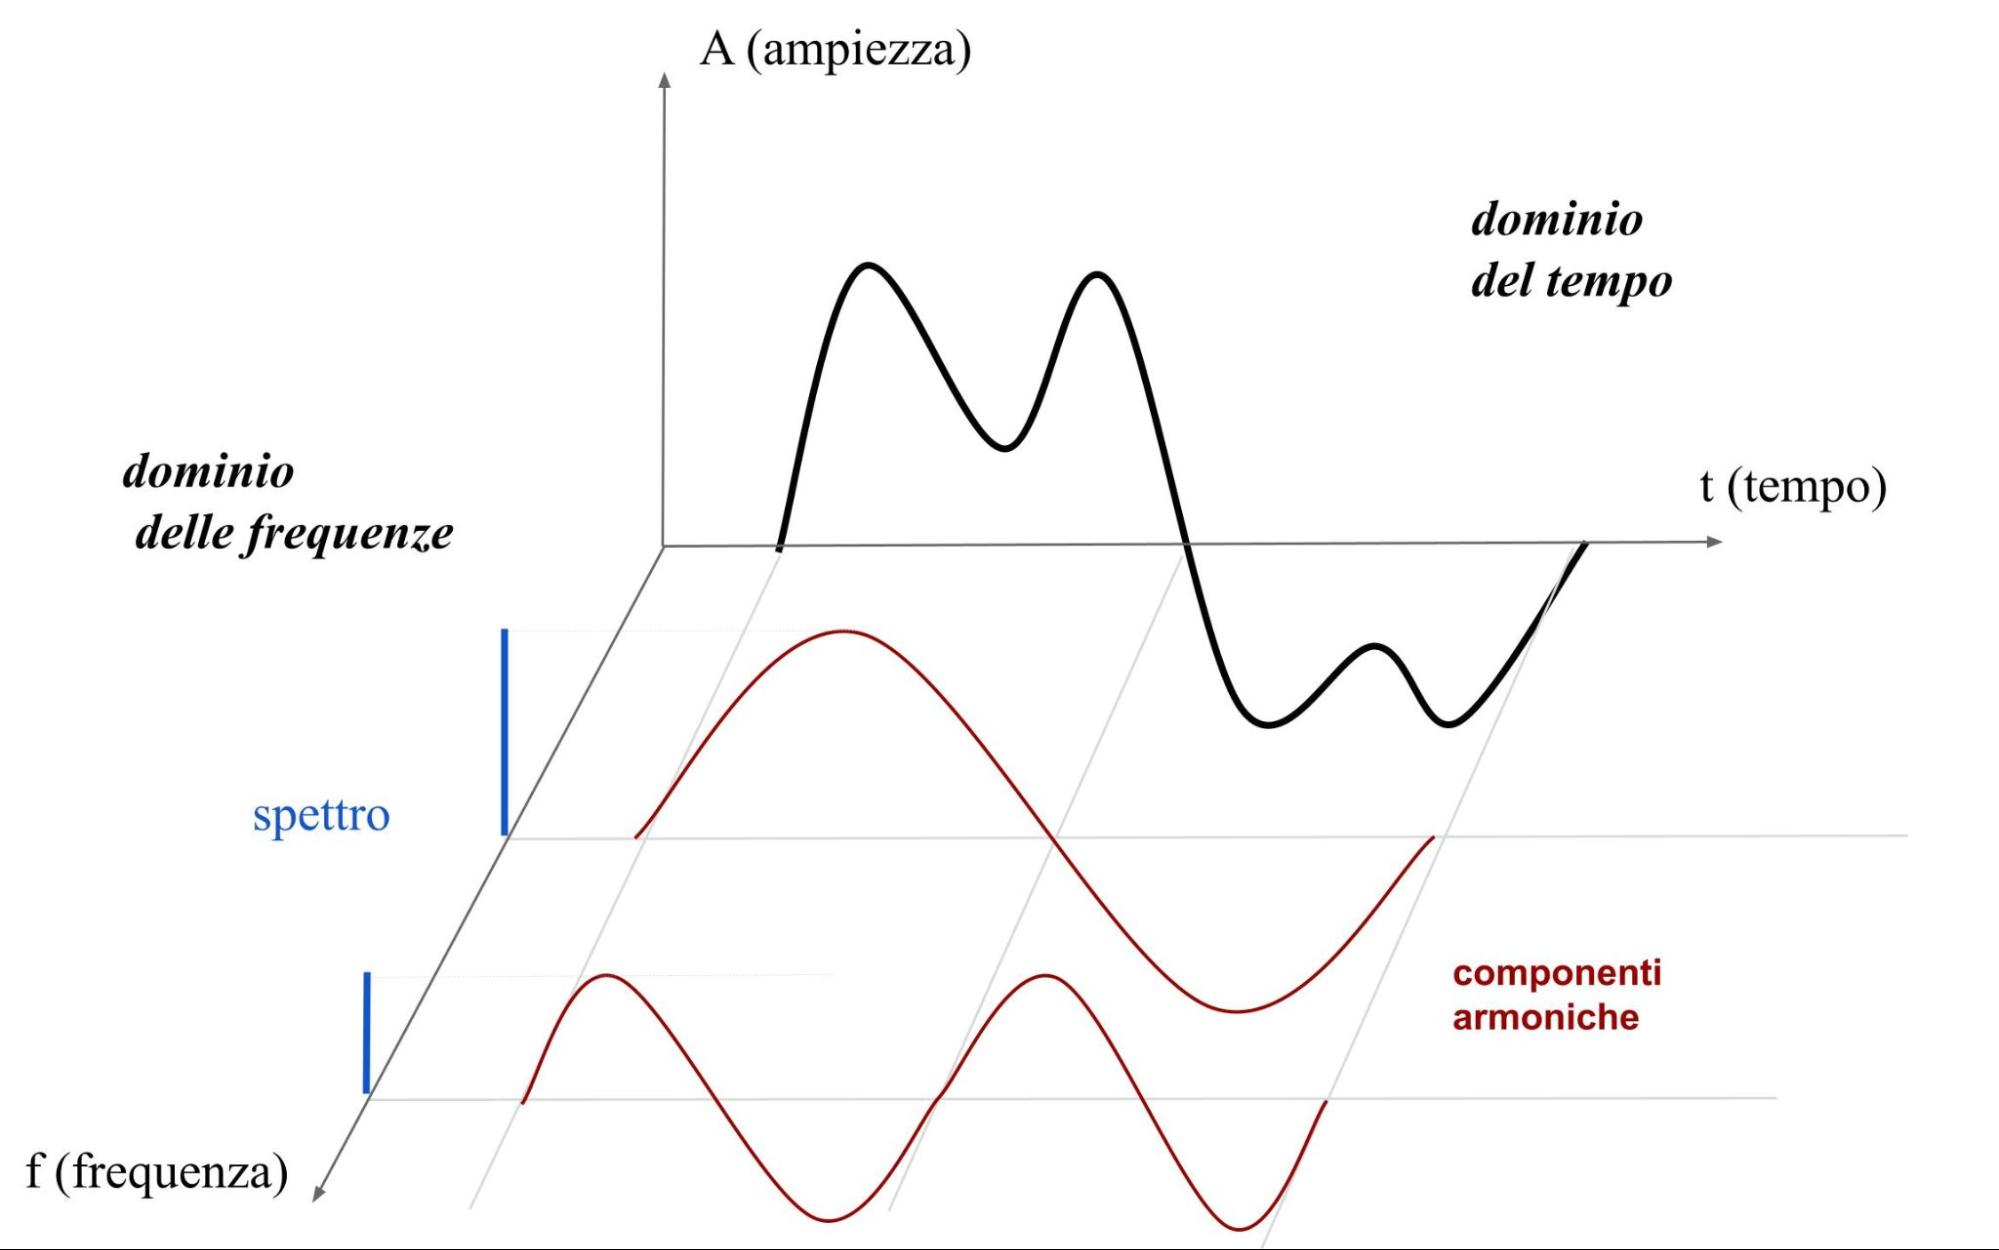
\includegraphics[width=0.9\textwidth]{img/cap2-dominioTempoFrequenza.jpg}
	\caption{Relazione tra dominio del tempo e dominio delle frequenze. In alto a destra la forma d’onda (in nero)
		rappresentata nel dominio del tempo in rapporto al tempo e all’ampiezza. Sotto le varie componenti armoniche
		dell’onda (forme ondulate in rosso). A sinistra viene rappresentato il dominio delle frequenze che presenta le
		ampiezze delle frequenze armoniche di cui è composta l’onda.} 
	\label{fig2.1}
\end{figure}
\begin{figure}[htp]
	\centering
	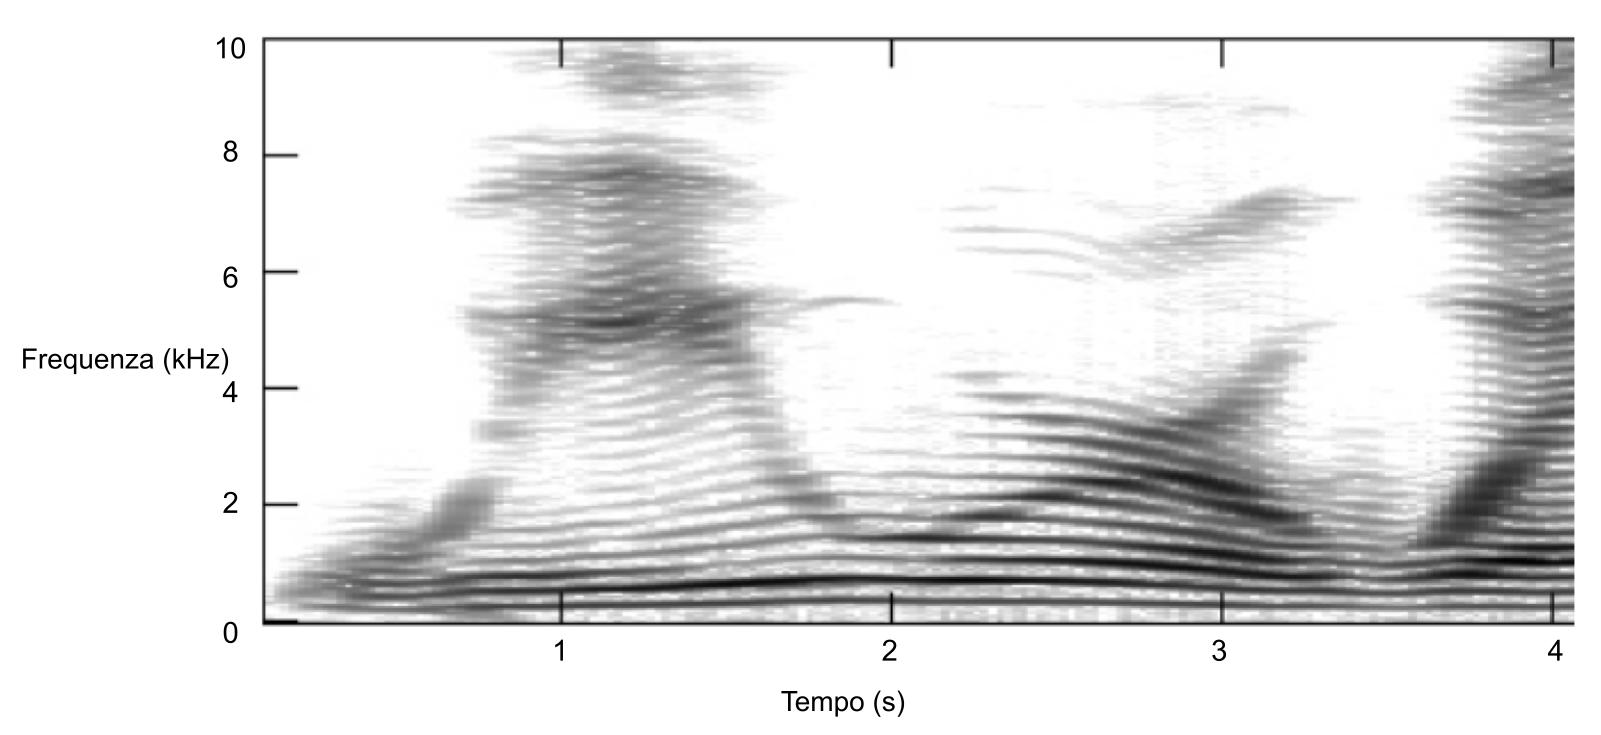
\includegraphics[width=0.9\textwidth]{img/cap2-spettrogramma.jpg}
	\caption{Spettrogramma di un file audio. Tale rappresentazione mostra come varia intensità nel tempo e nella frequenza. La scala di colori va dal bianco, che indica un'intensità sonora bassa, al nero, che rappresenta un'intensità sonora alta}
	\label{fig2.2}
\end{figure}

\clearpage
\section{Estrazione delle \textit{features}}
Distinguere due oggetti qualsiasi, come una bottiglia e una mela, può sembrare una capacità
comune, per nulla speciale. Questa abilità è frutto di un meccanismo che il nostro cervello
sviluppa attraverso l’esperienza e la conoscenza. Per ogni oggetto con cui interagiamo, la
mente elabora un insieme di caratteristiche in grado di descriverlo e lo esegue con una tale
velocità che nemmeno ce ne accorgiamo. Il cervello estrae elementi in grado di definire
l’oggetto, come il colore, la lunghezza e la forma, e con ogni senso del corpo. L’oggetto è da
intendersi anche come un profumo, un suono, un'immagine o qualsiasi altra percezione.

Al fine di insegnare questa capacità ad una macchina, è necessario identificare ciò che è
rilevante, discriminante e misurabile nei dati: le caratteristiche, o \textit{features}. Le \textit{features}
forniscono le informazioni necessarie per costruire il modello in grado di individuare i
\textit{pattern} nei dati e generalizzare, ovvero la capacità di riconoscere anche oggetti mai visti.

In questo studio, che tratta di \textit{soundscape}, l’oggetto da analizzare è un segnale audio. Per
caratterizzare tale segnale sono state utilizzate delle classiche misure di \textit{signal processing},
che si basano sui concetti illustrati nel paragrafo precedente.

Si possono distinguere tre gruppi principali di \textit{features}: spettrali (SPE), tonali (TON) e
temporali (TEM) [7].

Le SPE caratterizzano la forma dello spettro e influenzano le percezione del timbro. Tali
features vengono calcolate sullo spettrogramma del segnale. Si suddividono in:
\begin{itemize}
	\item{\textit{Spectral Centroid}: consiste nella media pesata delle frequenze nel segnale e indica il
		centroide, ovvero il centro di massa dello spettro. Valori più elevati indicano un suono
		più brillante [7]. Per brillante si intende che la maggioranza delle armoniche si trova
		su alte frequenze.}
	\item{\textit{Spectral Spread}: misura la dispersione delle frequenze attorno al centroide [7]. Un
		valore  basso indica una concentrazione maggiore delle frequenze attorno al centroide.}
	\item{\textit{Spectral Rolloff}: misura la frequenza al di sotto della quale si trova una percentuale
		specifica dell'energia totale dello spettro. Valori bassi indicano una scarsa presenza di
		componenti ad alte frequenze [7].}
	\item{\textit{Spectral Decrease}: misura quanto l’energia spettrale cala rapidamente all’aumentare
		delle frequenze. Un curva ripida indica una diminuzione rapida dell’energia spettrale,
		quindi un blocco ricco di basse frequenze e povero di alte frequenze [7].}
	\item{\textit{Spectral Flux}: rileva il numero di cambiamenti nella forma dello spettro. Identifica
		variazioni rapide e significative nel contenuto del segnale [7].}
\end{itemize}
Le TON misurano le componenti tonali del segnale rispetto al rumore. Tali feature vengono
calcolate sullo spettrogramma del segnale. Sono composte da:
\begin{itemize}
	\item{\textit{Spectral Crest Factor}: descrive il rapporto tra il valore massimo delle magnitudini
		dello spettro e la somma di tutte le magnitudini dello spettro (la magnitudo si riferisce
		all’ampiezza massima raggiunta da ogni frequenza nello spettro del segnale). Un
		valore basso indica un segnale molto uniforme [7].}
	\item{\textit{Spectral Flatness}: indica quanto lo spettro è uniforme. Un valore alto suggerisce un
			segnale con poca struttura tonale, quindi molti rumori.}
	\item{\textit{Spectral Tonal Power Ratio}: rapporta l’energia tonale con l’energia totale. Un valore
			alto indica che l’energia si concentra in componenti tonali, basso sui rumori [7].}
\end{itemize}
Infine le TEM, che descrivono come il segnale varia rispetto al tempo. Tali features vengono
calcolate sul segnale nel dominio del tempo. Si suddividono in:
\begin{itemize}
	 \item{\textit{Time Zero Crossing Rate}: identifica il numero di volte in cui il segnale cambia di
	 	segno quindi quando ha valore zero. Un valore alto indica una forte presenza di alte
	 	frequenze [7].}
	 \item{\textit{Time Acf Coeff}: quantifica la correlazione tra il segnale e una versione ritardata dello
	 	stesso (funzione di autocorrelazione). Questa misura è utile per identificare pattern
	 	ripetitivi [7].}
	 \item{\textit{Time Max Acf}: indica il valore massimo dell’autocorrelazione. Un valore alto può
	 	esprimere una forte periodicità del segnale [7].}
\end{itemize}	

\section{Standardizzazione dei dati}
La standardizzazione è un'attività di pre-processamento dei dati in grado di trasformarli in
una forma indipendente dalla scala utilizzata. Per scala si intende l’intervallo in cui le varie
\textit{features} vivono, ed è fondamentale per confrontare i dati. Infatti, una certa misurazione può
avere un rapporto diverso con gli altri dati a seconda della scala. Immaginiamo di avere i
risultati di due esami scolastici diversi, fatti da due gruppi di studenti. Il primo gruppo ha
ottenuto i risultati in centesimi, un intervallo da 1 a 100, invece il secondo gruppo, in
trentesimi, da 1 a 30. Un voto di 30 nel primo gruppo è molto diverso da un voto 30 nel
secondo gruppo: senza standardizzare la scala il confronto è falsato. Si deve quindi riportare
alla stessa scala. La standardizzazione è un insieme di tecniche dove vengono uniformate le
versioni ottenendo una versione standard dei dati, “senza dimensionalità”.

Una tecnica di standardizzazione molto utilizzata è lo \textit{Z-score standardization}, qui specificata
con la formula:
\begin{equation}
	x^{*}_{ji} = \frac{x_{ji} - \overline{x}_{j}}{\sigma_{j}}
\end{equation}
Si definisce \( x^{*}_{ji} \) la \textit{j}-esima \textit{feature} dell’oggetto \textit{i} standardizzata, 
\( x_{ji} \) la \textit{j}-esima feature dell’oggetto \textit{i} prima della standardizzazione, 
\( \overline{x}_{j} \) la media della \textit{feature} \textit{j} ed infine \( \sigma_{j} \) la 
deviazione standard delle \textit{features}. Si consideri ora una matrice composta sulle righe dagli
oggetti in esame e in colonna i valori delle \textit{feature}. Per ogni elemento \textit{x} in riga \textit{j} e posizione \textit{i} viene sottratta la media calcolata in colonna \textit{j}, e il valore ottenuto si divide con la deviazione
standard estratta dalla colonna \textit{j}. Dopo la standardizzazione ogni feature ha media uguale a 0
e deviazione standard a 1.

\section{Classificazione}
La classificazione è uno dei \textit{task} più utilizzati, affrontato con tecniche di PR e ML. Un
classificatore rappresenta un sistema decisionale in grado di assegnare una categoria, o
etichetta, ad un oggetto sulla base di un modello, tipicamente a partire da una descrizione
vettoriale (vettore di \textit{features}). In sostanza, è una funzione che prende in input un oggetto, ne
elabora le \textit{features} e restituisce un valore discreto che determina a quale categoria appartiene.

In generale gli approcci alla classificazione si suddividono in generativi e discriminativi.

Nell’approccio generativo si mira a definire un modello per ogni categoria, o classe. Questa
tipologia di approcci presenta una struttura più flessibile in grado di adattarsi a nuove classi, è
più rapida nell’addestramento e ottiene una migliore capacità descrittiva per la singola classe.

L’approccio discriminativo, invece, si basa sulla ricerca del migliore confine decisionale per
separare le classi nello spazio. Per sua natura è più rapido, soprattutto nella fase di test, e
presenta un'efficacia di classificazione migliore dato che il sistema viene costruito
specificatamente per risolvere il problema di classificazione.

Un'ulteriore suddivisione nei classificatori si basa sulla loro natura parametrica o non
parametrica. La parametrica si caratterizza per l’assunzione della forma di distribuzione dei
dati per ogni classe (es. la distribuzione normale), e si concentra nella stima dei parametri
della funzione che genera tale distribuzione. Diversamente, la non parametrica non assume
nessuna forma di distribuzione, ma viene stimata direttamente dal \textit{training set}. Risulta più
dispendiosa in termini computazionali ma non basandosi su assunzioni determina un modello
maggiormente flessibile e adattabile al contesto.

\subsection{Apprendimento supervisionato}
Nella PR spesso si utilizza il paradigma dell’\textit{apprendimento da esempi}. Questo metodo può
essere visto come l’apprendimento di un bambino che sperimenta e acquisisce conoscenza da
esempi, dall’esperienza. In particolare, nel contesto della classificazione, si utilizza un
approccio supervisionato in cui la conoscenza viene acquisita tramite dati campionati dal
problema, il \textit{training set}, dotato di categorie, o etichette, note. Conoscendo la reale classe di
appartenenza degli oggetti, il modello può addestrarsi e migliorare gradualmente la sua
capacità di classificazione. In questo processo è importante che il sistema non “impari a
memoria” i dati del \textit{training set}, il cosiddetto \textit{overfitting}, che comporta un eccessivo
adattamento ai dati di addestramento. L’obiettivo infatti è di creare un modello in grado di
generalizzare quindi di classificare correttamente anche oggetti sconosciuti, mai visti.

\subsection{Validazione}
Una volta costruito il modello è necessario verificare la qualità del classificatore. Per tale
scopo si utilizza il \textit{testing set}, un \textit{dataset} che presenta elementi diversi da quelli usati in
addestramento, ma dotato di categorie note da confrontare con il risultato predetto dal
classificatore. Il modello classifica tali dati e si valuta la predizione in base all’errore
ottenuto. Questo valore pone in rapporto le previsioni errate rispetto al numero totale di
oggetti analizzati. Una previsione errata consiste in una falsa valutazione del classificatore,
quindi un valore diverso dalla reale categoria di appartenenza.

Nella costruzione di un classificatore di solito si dispone di un unico \textit{dataset} che si deve
suddividere in due parti, il \textit{training set}, per l’addestramento, e il \textit{testing set} per i test e la
validazione. Un metodo ideale sarebbe poter usare tutti dati di esempio per il \textit{training} ed
estrarre altri esempi dal problema per testare il modello, ma nella realtà potrebbe essere non
fattibile o troppo dispendioso. Si preferisce quindi usare una metodica comune che consiste
nella \textit{cross validation}, che permette di ottenere una valutazione più valida e consistente.
Esistono diverse varianti, ognuna con le sue caratteristiche. La forma più semplice è la
\textit{Holdout}, che distribuisce casualmente i dati in due insiemi di uguale dimensione.
Un'alternativa simile è l’\textit{Average Holdout}, che per essere indipendente dalle partizioni effettua
più \textit{holdout} e calcola l’errore come media dei risultati ottenuti in tutti i casi.

Infine, una delle più utilizzate è la \textit{Leave One Out} (LOO), una variante particolare che ottiene
ottimi risultati in termini di affidabilità, soprattutto con dataset ristretti. Come suggerisce il
nome, consiste nell’effettuare l’addestramento con tutti gli oggetti del \textit{dataset} meno uno, 
\( x_{i} \), che viene invece utilizzato per validare il modello. Si ripete il procedimento lasciando fuori
come oggetto di testing un diverso elemento \( x_{i} \) del \textit{dataset}, e al termine si media il risultato
ottenuto. Presenta un costo computazionale maggiore ma garantisce indipendenza dalla
partizione e dai dati scelti del \textit{training set} e \textit{testing set}.

\subsection{Metodo di classificazione}
In questo studio è stato utilizzato il classificatore \textit{K Nearest Neighbor} (KNN), un approccio
supervisionato generativo non parametrico, semplice e intuitivo: il metodo si basa sul
classificare un punto, un oggetto, assegnandogli la classe che più frequentemente ritroviamo
tra i \textit{k} oggetti più vicini. Il concetto di vicinanza si concretizza con la scelta della distanza: nel
nostro caso la \textit{distanza euclidea}, una delle misure più utilizzate. Come risulta chiaro, la scelta
del valore di \textit{k} è cruciale.


\section{Anomaly Detection}
L’\textit{anomaly detection} (AD) consiste nell’identificare fenomeni ed eventi che presentano un
comportamento anomalo rispetto al resto del \textit{dataset} [8]. Tali fenomeni, denominati \textit{outlier}, si discostano in modo significativo dagli \textit{inlier}, il resto dei dati normali, per la loro natura anomala e la scarsa numerosità.

\begin{figure}[htp]
	\centering
	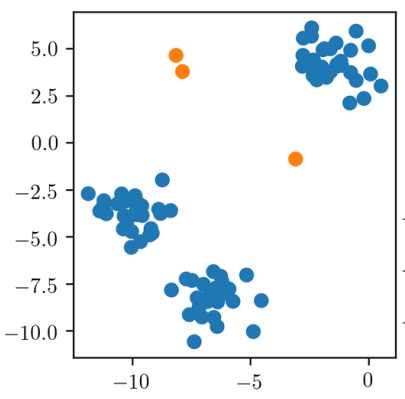
\includegraphics[width=0.4\textwidth]{img/cap2-AnomalyDetection.png}
	\caption{Rappresentazione di \textit{inliers} (cerchi colore blu) e outliers (cerchi colore giallo) in un \textit{dataset}. Si nota come gli \textit{outlier}, in questo caso, risultano distaccati dal comportamento generale definito dagli inlier, che sono raggruppati e seguono una distribuzione più omogenea.}
	\label{fig2.3}
\end{figure}

\subsection{Gli \textit{outlier}}
Individuare gli \textit{outlier}, pur essendo complicato, è una necessità. Ciò consentirebbe di inferire
informazioni preziose oppure rappresentare una prevenzione per eventuali criticità.
Contribuisce in modo significativo anche al data cleaning, la “pulizia dei dati”, che conta di
un insieme di processi che servono a rimuovere duplicati, uniformare e filtrare i dati. In
questo contesto rimuovere gli outlier semplificherebbe le fasi successive di analisi
migliorando la qualità del risultato.

Si distinguono varie tipologie di \textit{outlier}:
\begin{itemize}
	\item{i \textit{point}, che sono identificati tali indipendentemente se si trovano da soli o in gruppo;}
	\item{i \textit{collective}, considerati outlier solo se rilevati in gruppo, altrimenti rientrano negli \textit{inlier};}
	\item{i \textit{contextual}, che sono rilevati normali o anomali in base al contesto specifico in cui si
	trovano. Per esempio, in un sistema di monitoraggio della temperatura di una città,
	una valore di 30 gradi durante l’estate verrà considerato normale, diversamente lo
	stesso valore in inverno sarà definito anomalo.}
\end{itemize}

\subsection{Le applicazioni}
L’AD ricopre un ruolo importante in molteplici campi. Per esempio, possiamo citare:
\begin{itemize}
	\item{le intrusioni di rete: in un rete informatica di sistemi che condividono informazioni
	monitorare attività sospette o non autorizzate è fondamentale. Tali attività, come un
	programma o un individuo malevole, potrebbero insinuarsi con lo scopo di rubare dati
	o compromettere la sicurezza. Sistemi basati su AD consentono di rilevare tali
	comportamenti come anomali poiché si discostano dal traffico della rete considerato
	normale;}
	\item{l’ambito sanitario: fondamentale nell’analisi dei dati dei pazienti per diverse ragioni
	come condizioni di salute anomale, errori nella strumentazione o nelle registrazioni
	mediche. Tale approccio potrebbe contribuire in modo significativo nel rilevamento di
	situazioni potenzialmente critiche, sia per intervenire in anticipo che per evitare errori
	nella diagnosi;}
	\item{i sistemi automatizzati, in cui prevenire un avaria o, riuscire a intervenire in tempo nel
	caso si manifestasse, è essenziale;}
	\item{nel processamento di immagini o testi, come rilevare \textit{fake news};}
	\item{nel rilevamento di frodi, all’interno delle innumerevoli transazioni bancarie prodotte
	ogni giorno.}
\end{itemize}
Queste casistiche sono accomunate da un enorme quantità di dati dove sistemi troppo rigidi e
specifici non potrebbero adattarsi al continuo mutamento delle variabili in gioco. Le
problematiche nell’AD sono svariate. I contesti affrontati non sono supervisionati, non vi è
modo di basarsi su esempi espliciti di \textit{outliers} dato che non esiste una chiara definizione di
ciò che rende un'anomalia tale e il rischio di determinare falsi positivi è molto alto.

\subsection{I metodi}
I diversi approcci di AD tipicamente si suddividono sulla base del metodo utilizzato per
rilevare le anomalie. I vari metodi possono essere:
\begin{itemize}
	\item{Metodi basati sui concetti statistici: essi ricercano elementi che non rispecchiano la
		distribuzione dei dati. Una bassa probabilità di appartenenza alla distribuzione
		determina un'alta probabilità di essere un \textit{outlier}.}
	\item{Metodi basati sul \textit{clustering}: essi suddividono i dati per somiglianza in gruppi, i
		cluster, e le anomalie risultano evidenti poiché molto diverse dal loro gruppo di
		appartenenza. Oppure gli \textit{outlier} formano piccoli cluster che presentano una
		dimensione o una densità inferiori alla soglia necessaria per essere considerati tra i
		dati normali, venendo quindi identificati come anomalie.}
	\item{Metodi basati sull’apprendimento: vengono utilizzati metodi di apprendimento
		automatico per ricercare \textit{pattern} all’interno dei dati. Gli elementi che non si
		identificano in questi \textit{pattern} vengono considerati come anomalie.}
	\item{Metodi basati sulla distanza o sulla densità: viene considerata la distanza tra gli
		elementi, o la densità locale. Nel primo caso gli \textit{outlier} si troveranno distanti dagli
		altri punti, nel secondo saranno in zone a bassa densità.}
	\item{Metodi basati sulla combinazione di vari metodi, o \textit{ensemble}: queste tipologie
		combinano i risultati di metodi diversi, o gli stessi con parametri differenti, per
		ottenere una previsione più accurata.}
\end{itemize}	
La maggioranza degli algoritmi ritorna come risultato un valore, denominato \textit{Anomaly score},
che quantifica quanto un elemento è probabile che sia un’anomalia.

In letteratura esistono differenti algoritmi di AD [8], ma di seguito ne saranno descritti solo
tre, quelli utilizzati nello studio. I metodi sono L’\textit{IForest} (IF) [9], o \textit{Isolation forest}, il \textit{Local Outlier Factor} (LOF) [10] e l’\textit{Ocsvm} (OCSVM) [11], o \textit{One Class Support Vector Machine}.

IF è un algoritmo basato su un \textit{ensemble} [8] di alberi decisionali. Per albero decisionale si
intende una struttura ad albero dove ogni nodo contiene un test e i rami le possibili risposte.
Procedendo dall’alto verso il basso del modello, i dati vengono indirizzati dalle varie risposte
fino alle foglie, lungo il path. In IF viene costruita una foresta di alberi decisionali e ciascun
albero cerca di isolare i dati mediante suddivisione. L’idea è che le anomalie avranno un path
più corto poiché avranno bisogno di meno divisioni rispetto ai dati normali. In sostanza, più
risulta facile isolare un oggetto e con maggiore probabilità sarà un anomalia. Questo
algoritmo risulta molto scalabile, veloce e accurato, specialmente su dataset di grandi
dimensioni.

LOF è un metodo basato sulla densità. La densità di un oggetto può essere calcolata
guardando al suo vicinato, ovvero dalla numerosità degli elementi che gli sono vicini. Il
criterio utilizzato per determinare la vicinanza ad un oggetto dipende dalla metrica scelta
nell’implementazione. La più comune è la distanza euclidea, che misura la lunghezza del
segmento tracciato tra due punti. In sostanza, l’algoritmo stabilisce che minore è la densità
locale allora più alta è la probabilità che un determinato oggetto possa essere un’anomalia.
Questo metodo è efficace con dati ad alta dimensionalità, ma al contrario, risulta molto
dispendioso in termini computazionali.

Infine, OCSVM si basa sull’apprendimento. Si tratta di una variante delle \textit{Support Vector Machine}, un approccio discriminativo applicato solitamente a problemi binari. In questa
forma, a singola classe, l’algoritmo viene addestrato per definire un confine che racchiude al
suo interno solo i dati normali. Così facendo i dati anomali, che risultano esterni alla
distribuzione, emergono e sono quindi rilevabili. Spesso viene utilizzato il trucco del \textit{kernel},
che consiste nel proiettare i dati in una dimensione superiore, dove può risultare più facile
separare i dati.	
	\clearpage\cleardoublepage\chapter{Dataset}
Lo studio condotto si è basato sui dati raccolti nell’ambito di un monitoraggio acustico
passivo nella \textit{Riserva Naturale Los Yátaros}, nel dipartimento di \textit{Boyacá} in \textit{Colombia} [3]. Con il termine passivo si identifica una modalità di osservazione del paesaggio incentrata sulla
registrazione di un particolare luogo e solo successivamente prevede un’analisi approfondita,
diversamente da quella attiva, dove si osserva e si analizza il fenomeno in tempo reale. La
raccolta dati è stata commissionata dalla fondazione \textit{Von Humboldt}, un ente colombiano che
si occupa di ricerca sulla biodiversità e sulle sue relazioni con il benessere umano.

La riserva è composta da querceti e foresta subandina in diversi stadi di rigenerazione
naturale, e presenta una biodiversità acustica molto particolare. Il progetto mirava a profilare
l’impronta acustica della riserva campionando suoni nello spettro udibile e negli ultrasuoni.

Sono stati predisposti tre siti, denominati \textit{YAT}, organizzati in una disposizione triangolare,
lungo il sentiero principale, distanti 150 m, con due sensori acustici \textit{AudioMoth} ciascuno, per
le due forme di suono desiderate, posti ad altezza diverse. Il periodo di campionamento si è
svolto dall’1 marzo al 2 maggio 2020, registrando un minuto di audio ad intervalli di trenta
minuti durante tutto il giorno (dalle 00:00 alle 23:30) per lo spettro dell’udibile (0 \textit{Hz} - 16 \textit{kHz}) e nella fascia notturna (dalle 16:30 alle 6:00) per lo spettro dell’ultrasuono (fino a 192 \textit{kHz}). In totale si è ottenuto 12447 registrazioni di cui 9055 nell'udibile e 3392 nell’ultrasuono. In questo progetto, sono stati considerati solo i dati nello spettro udibile, per permettere l’ascolto del contenuto.

\section{Dataset prima fase}
Nella prima fase dello studio è stato utilizzato il \textit{dataset} completo (DATA1) che presenta
l’insieme originale dei dati. Il gruppo si presenta con una suddivisione per i tre siti (YAT1,
YAT2, YAT3) con quantità leggermente differenti. Gli audio sono 3018 per \textit{yat}, a parte il
primo con 3019. Ogni sito presenta 1482 file per il mese di marzo (1483 solo per YAT1),
1440 per il mese di aprile e 96 per il mese di maggio.

Data l’ingente quantità di dati disponibile, non si è potuto analizzare il contenuto, ossia
ascoltare l’intero insieme di registrazioni. In una prima caratterizzazione, analizzando diversi
audio in momenti diversi della giornata e del mese, si è osservato che tutti e tre i luoghi 
risultano molto caratterizzati dal suono del fiume e della cascata vicina. È importante notare
che anche se tale suono fosse stato ad una distanza maggiore avrebbe sortito lo stesso effetto:
infatti Farina \textit{et al.} sostengono che “la geofonia può essere rilevata anche a grandi distanze in
base all’ampiezza della sorgente sonora” [3]. A questo si aggiungono ulteriori problematiche
dovute a periodi piovosi, il cui rumore sovrasta in diverse occasioni i suoni ambientali
naturali. Entrambi gli elementi appena descritti determinano un ambiente umido che potrebbe
influire anche sulla capacità del sensore.


\section{Dataset seconda e terza fase}
Il \textit{dataset} della seconda e terza fase dello studio (DATA2) consiste in un sottoinsieme del
\textit{dataset} DATA1. Per potere inferire maggiori informazioni dal contesto si è stabilito che era
necessaria una descrizione più accurata del contenuto. Quindi si è ristretto l’insieme ad un
campione di dati minore che potesse essere ascoltato e studiato nel dettaglio. L’analisi ha
estratto dal \textit{dataset} originale 186 audio, focalizzandosi sul sito YAT1, nel mese di marzo con
finestre temporali a intervalli di due ore, partendo dalle due del mattino, quindi nelle ore:
02:00, 06.00, 10:00, 14:00, 18:00, 22:00. Con questa modalità si può ottenere una visione
abbastanza generale della varietà sonora presente nella giornata, includendo i due momenti
fondamentali di alba e tramonto, caratterizzati da picchi di attività acustica.

L’interpretazione manuale del \textit{dataset} ha classificato il contenuto assegnando delle etichette
ai vari elementi distinti utilizzando i gruppi delle categorie descritte nel paragrafo 1.1. In relazione
all’ANT è stato individuato un unico suono, appartenente al rumore di veicoli (classe V).
Nella BIO è stato individuato il verso degli uccelli e dei grilli (classi U e G). Per la GEO si è
rilevato il precedentemente menzionato rumore del fiume/cascata, la pioggia e i tuoni (classi
C, P e T). Infine, sono stati identificati i rumori relativi alle interferenze del sensore (classe I),
ed eventuali elementi uditi ma non interpretati (sconosciuti classe S) . Rispetto a quanto
specificato nell’introduzione, all’interno della GEO si è integrato anche l’insieme dei suoni
relativi alla quiete. Tale scelta è derivata da una maggiore semplicità nella trattazione, ma
specialmente per l'impossibilità nel poterli classificare correttamente.

Nel grafico della figura 3.1 è possibile visualizzare la distribuzione degli elementi descritti nelle fasce
analizzate. Da una prima osservazione risulta evidente la significativa presenza dell’elemento
C, come già esplicitato nel paragrafo precedente. Lo stesso comportamento si può osservare
al suono dell’elemento U, risultato meno attivo solo nella parte centrale della giornata. Il
resto è relativamente distribuito, a parte I e S diffusi con bassa intensità. Si può notare come
S sia presente solo nelle due fasce pomeridiane. Dal grafico della figura 3.2 possiamo avere una
prospettiva alternativa della distribuzione di ogni suono su tutto il mese di marzo, per il quale
è lecito esplicitare le medesime considerazioni annotate.

\hfill
\begin{center}	
\begin{figure}[htp]
	\centering
	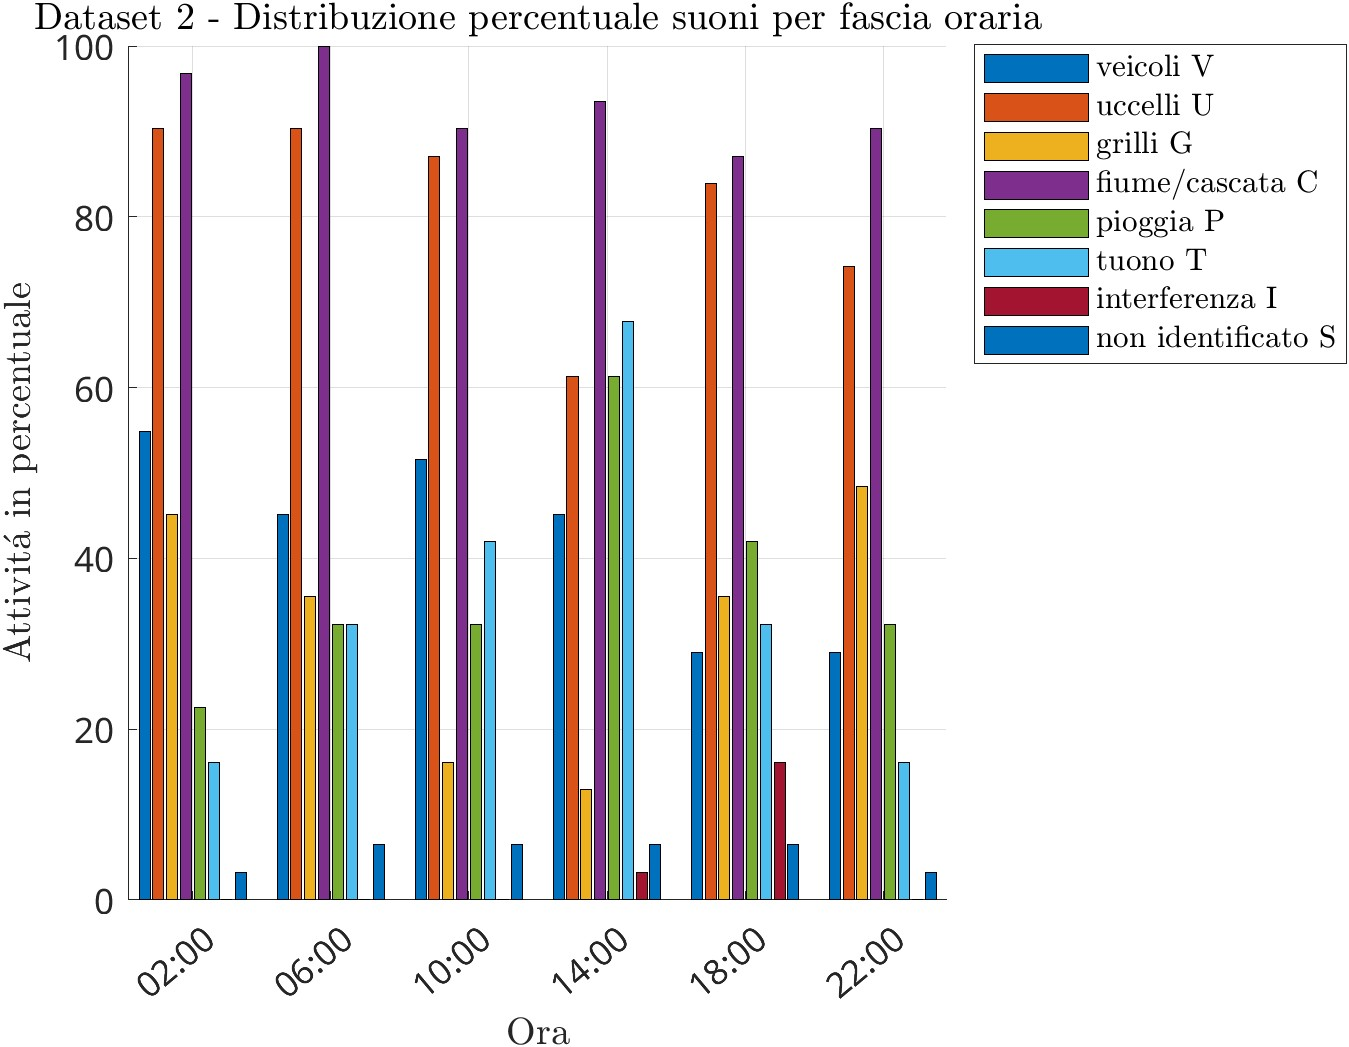
\includegraphics[width=0.9\textwidth]{img/cap3-dataset1.jpg}
	\caption{Esposizione della presenza sonora in percentuale per ogni suono nelle varie fasce orarie.}
	\label{fig3.1}
\end{figure}
\end{center}
\begin{center}
\begin{figure}[htp]
	\centering
	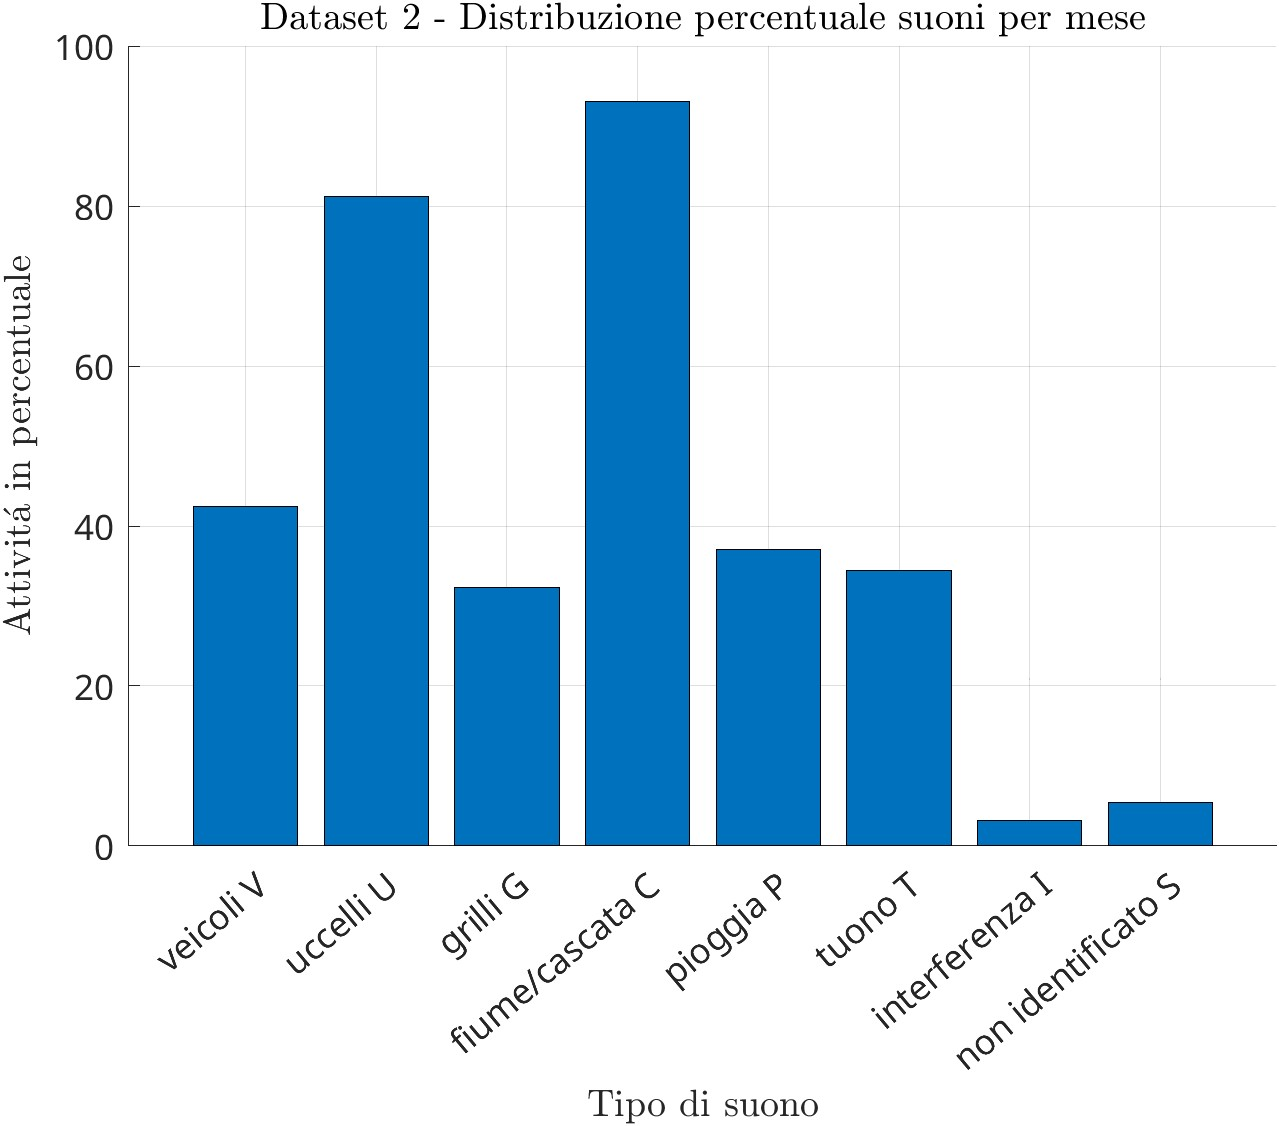
\includegraphics[width=0.8\textwidth]{img/cap3-dataset2.jpg}
	\caption{Esposizione della presenza sonora in percentuale per ogni suono in tutto il mese. Ogni suono
		presenta un percentuale di distribuzione su tutti gli audio analizzati. Si tiene in considerazione che ogni audio può contenere più suoni.}
	\label{fig3.2}
\end{figure}
\end{center}
	\clearpage\cleardoublepage\chapter{Classificazione}
In questo capitolo verranno descritti i risultati relativi alle prime due fasi dello studio basate
sulla classificazione: la prima riguardante la classificazione su categorie oggettive, la seconda
su categorie semantiche. Le categorie oggettive riguardano informazioni deducibili dai
metadati dei file audio, come il luogo di registrazione o una fase della giornata. Le categorie
semantiche invece si riferiscono a informazioni ricavate dall’analisi del contenuto dell’audio,
ovvero ai vari suoni identificati presenti nella foresta.

Saranno definiti i gruppi di features utilizzati negli esperimenti, descrivendo poi la tipologia
di classificatore scelto. A seguire, saranno illustrati nel dettaglio i problemi di classificazione
disegnati, ed infine si andrà ad analizzare i risultati ottenuti nei due esperimenti.
L’obiettivo è determinare la parametrizzazione migliore per l’approccio, quali features sono
più efficaci al nostro contesto, e in quali problemi ottengono i risultati migliori. Questo studio
considera gli esperimenti di classificazione precedentemente condotti dai colleghi Ilaria
Ballerini e Andrea Piazza.

Inoltre, viene analizzata la possibilità di aggiungere una fase di filtraggio per alcune
frequenze. L’idea consiste nel rimuovere alcune frequenze preponderanti su ogni audio, che
rappresentano rumore, dovute in maggior parte alle problematiche intrinseche del contesto,
ma anche alla sensibilità dello strumento di misurazione.

\section{Configurazioni \textit{features}}
Nello studio sono state considerate sia le \textit{features} nella loro forma originale, come descritta
nel paragrafo 2.2, sia aggregate. Le \textit{features} originali sono descritte da un numero definito di
componenti (che saranno indicate con \textit{N}). Ogni feature originale è quindi descritta da un
vettore riga di 1x\textit{N} componenti. N dipende dai parametri usati per calcolare lo
spettrogramma.

In particolare sono stati identificati 19 gruppi di \textit{features}:
\begin{itemize}
	\item{11 ORIGINALI (o ORIG), per ognuna delle 11 \textit{features}, utilizzate singolarmente, 1x\textit{N} elementi ciascuna;}
	\item{CONCATENAZIONE ORIGINALI (o CONC.ORIG.), formata dalla concatenazione
	orizzontale delle 11 \textit{features} originali, ottenendo un totale di 11x\textit{N} componenti;}
	\item{CONCATENAZIONE SPETTRALI (o CONC.SPE.), ottenuta dalla concatenazione
	delle componenti delle 5 \textit{features} spettrali, quindi 5x\textit{N} componenti;}
	\item{CONCATENAZIONE TONALI (o CONC.TON.), come la precedente ma
	considerando le 3 \textit{features} della tonalità, ovvero 3x\textit{N} componenti;}
	\item{CONCATENAZIONE TEMPORALI (o CONC.TEM.), come la precedente ma con le
	3 \textit{features} temporali, 3x\textit{N} componenti;}
	\item{CONCATENAZIONE MEDIE ORIGINALI (o CONC.MED.ORIG.), formata dalla
	concatenazione orizzontale delle medie delle 11 \textit{features} originali, quindi 11
	componenti;}
	\item{CONCATENAZIONE MEDIE SPETTRALI (o CONC.MED.SPE.), ottenuta dalla
	concatenazione orizzontale delle medie delle componenti delle 5 \textit{features} spettrali,
	quindi solo 5 componenti;}
	\item{CONCATENAZIONE MEDIE TONALI (o CONC.MED.TON.), come la precedente
	ma utilizzando le 3 \textit{features} tonali, quindi solo 3 componenti;}
	\item{CONCATENAZIONE MEDIE TEMPORALI (o CONC.MED.TEM.), come la
	precedente ma utilizzando le 3 \textit{features} temporali, in totale 3 componenti;}
\end{itemize}

Ai 19 gruppi sopracitati si è tenuto conto anche della relativa versione standardizzata, ovvero
ottenuta dalle componenti processate con la tecnica di standardizzazione \textit{Z Score}, definendo
quindi 38 gruppi: 19 originali e 19 standardizzati. In questo modo, si dispone anche di una
rappresentazione con una scala comune indipendente dalle misurazioni originali.

In aggiunta, i dati sono stati estratti in due forme diverse (ottenendo quindi 78 gruppi di
\textit{features}) basate su diverse finestre temporali scelte per il campionamento nel calcolo dello
spettrogramma: la prima, FS0X, usa una finestra di 32768 campioni, quindi meno di 1
secondo; la seconda, FS1, invece si basa su una finestra di 48000 campioni, corrispondente a
1 secondo.

Nel caso di FS1 sono state estratte 120 componenti (\textit{N}=120): il segnale audio analizzato
presenta una lunghezza temporale di 60 secondi e, per costruire lo spettrogramma lo si
analizza con un intervallo di 1 secondo alla volta, ottenendo 60 finestre. Inoltre, considerando
un passo pari alla metà dell’intervallo, 0.5 secondi, si ottengono altre 60 finestre, per un totale
di 120 campionamenti. Alla stessa modo, è stato fatto per la configurazione FS0X dove,
considerando una finestra più breve, si è ottenuto un maggior numero di componenti
(\textit{N}=176).

La tabella 4.1 riassume i vari gruppi di features considerati.

\begin{table}[htp] 
	\centering
	\begin{tabular}{llrr}
		\toprule
		\textbf{Gruppi}  
		& \textbf{Descrizione}
		& \textbf{\# N x \textit{feature}}
		& \textbf{\# N x \textit{feature}} \\ 
		\textbf{di \textit{features}}
		&  \textbf{\textit{features}} 
		& \textbf{caso FS0X}
		& \textbf{caso FS1} \\
		\midrule
		CONC.ORIG. & Concatenazione originali & 1320 & 1936 \\
		CONC.SPE. & Concatenazione spettrali & 600 & 880 \\
		CON.TON. & Concatenazione tonali & 360 & 528 \\
		CONC.TEM. & Concatenazione temporali & 360 & 528 \\
		CONC.MED.ORIG. & Concatenazione medie originali & 11 & 11 \\
		CONC.MED.SPE. & Concatenazione medie spettrali & 5 & 5 \\
		CONC.MED.TON. & Concatenazione medie tonali & 3 & 3 \\
		CONC.MED.TEM. & Concatenazione medie temporali & 3 & 3 \\
		ORIG & Spectral Centroid & 120 & 176 \\
		ORIG & Spectral Crest Factor & 120 & 176 \\
		ORIG & Spectral Decrease & 120 & 176 \\
		ORIG & Spectral Flatness & 120 & 176 \\
		ORIG & Spectral Flux & 120 & 176 \\
		ORIG & Spectral Roll off & 120 & 176 \\
		ORIG & Spectral Spread & 120 & 176 \\
		ORIG & Spectral Tonal Power Ratio & 120 & 176 \\
		ORIG & Time Zero Crossing Rate & 120 & 176 \\
		ORIG & Time Acf Coeff & 120 & 176 \\
		ORIG & Time Max Acf & 120 & 176 \\
		\bottomrule		
	\end{tabular}	
	\caption{Elenco delle varie \textit{features} utilizzate con relative componenti nelle due configurazioni. Il simbolo \#
		rappresenta la numerosità.}
\end{table}

\section{Dettagli classificatore}
Il classificatore KNN è stato configurato con il valore più semplice, con \textit{k} uguale a 1, facile da
implementare e da comprendere, poiché la decisione della classe si basa unicamente
sull’elemento più vicino (comunemente viene indicata con solo \textit{1-NN}, o solo \textit{NN}). A suo
svantaggio, un valore troppo piccolo, come nel nostro caso, lo rende molto sensibile al
rumore, determinando risultati errati o incongruenze, influenzando l’accuratezza del modello.
Le performance del modello sono state valutate mediante la tecnica di cross validation \textit{Leave
One Out} (LOO). Per semplicità il sistema di classificazione sarà indicato con LOO KNN.

\section{Problemi di classificazione disegnati}
I due problemi di classificazione di questo studio hanno caratteristiche diverse che
illustreremo nei prossimi paragrafi, ma in sostanza si differenziano dalla tipologia di etichette
scelte: la prima cerca di separare classi di natura oggettiva (per esempio il giorno dalla notte),
la seconda invece classi di natura semantica.

\subsection{Problemi con categorie oggettive}
La prima fase propone uno studio sul \textit{dataset} DATA1. Il dataset è privo di annotazione ma
optare per un etichettatura manuale, identificando i vari suoni all’interno, non è considerabile,
sia per l’eccessivo tempo necessario che per la mancanza di risorse. Infatti, come specificato
nell’introduzione, i limiti più ostici consistono da una parte nella difficoltà oggettiva
intrinseca di discriminare elementi all’interno di un \textit{soundscape} e, dall’altra, nella
competenza tecnica necessaria a identificare la biodiversità presente. Per questi motivi, si è
deciso di studiare dei problemi basati su caratteristiche oggettive, cioè su informazioni
deducibili dal contesto dell’oggetto, invece che dal suo contenuto: ad esempio si è tenuto
conto del luogo di registrazione, e della temporalità, come l’ora del giorno, o una fase della
giornata, o del mese.

Sono stati individuati i seguenti problemi:
\begin{itemize}
\item{PR-1.1 YAT. L’obiettivo è individuare il luogo di registrazione, gli \textit{yat}. Si tratta di una
classificazione multiclasse, nel nostro caso 3, relative alle 3 zone in cui sono stati
collocati i microfoni. La cardinalità delle classi vede un 33\% di presenza per ognuno.}
\item{PR-1.2 G/N. Un problema binario che consiste nel discriminare le due fasi
astronomiche principali del giorno, classe G e della notte, classe N. In base alla
latitudine, è stata considerata la fascia oraria del giorno tra le ore 6 e le 17, estremi
compresi. Le ore restanti sono assegnate alla rispettiva classe che identifica la notte.
In tale problema le classi sono equamente bilanciate. }
\item{PR-1.3 AT/R. Un altro problema studiato che considera in un classe i suoni presenti
all’alba e al tramonto, classe AT, e nella seconda le ore rimanenti, classe R. La fascia
oraria considerata per alba è stata identificata tra le ore 5 e le ore 7, estremi compresi,
per il tramonto invece tra le ore 18 e le 20, estremi compresi. L’idea alla base dello
studio di questo problema è che nella prima classe ci possano essere dei suoni
caratterizzanti e simili rispetto al resto della giornata, riconoscibili nell’alba come il
risveglio della natura e nel tramonto come il calare della quiete. Quinn \textit{et alii}
evidenziano l’attività della biofonia in tali fasce della giornata [2]. In questa casistica
la distribuzione si trova in parte sbilanciata sulla classe R, presente per un 70\%.}
\item{PR-1.4 A/T/G/N. Si tratta di una classificazione multiclasse, composta da 4 classi,
discriminando alba, classe A, tramonto, classe T, e le ore rimanenti diurne e notturne,
classi G e N. Le fasce orarie per l’alba e il tramonto sono le medesime presentate
sopra. Le classi A e T sono in una percentuale di distribuzione minore, con circa un
15\% cadauna, rispetto alle classi G e N, che presentano un valore di 40\% e 30\%.}
\item{PR-1.5 M. Problema a 3 classi, che mira a identificare i relativi mesi in cui sono stati
registrati i dati. Per il terzo mese, maggio, è presente un forte squilibrio dovuto alla
mancanza di dati, che si identifica con solo un 4\% dei dati, rispetto a marzo e aprile
con il 49\% e 47\%.}
\item{PR-1.6 MM. Problema binario che mira a discriminare la prima parte del mese (da
inizio mese fino al quindicesimo giorno) dalla seconda (dal sedicesimo giorno fino a
fine mese). La distribuzione è ottimamente bilanciata con circa il 50\% per entrambe le
classi. }
\end{itemize}

In alcune casistiche i dati presentano parti sbilanciate che potrebbero inficiare sulla qualità
del risultato: riguarda maggiormente il problema PR-1.5 M che soffre di una componente poco
rappresentata, il mese di maggio. In questo studio non sono state considerate delle tecniche
conosciute in letteratura per compensare il divario, tuttavia sarebbe sicuramente un aspetto
interessante da esplorare in studi futuri.

\subsection{Problemi con categorie semantiche}
La seconda fase utilizza il \textit{dataset} DATA2, sottoinsieme del \textit{dataset} principale. Come
precedentemente descritto nel capitolo 3, riducendo il set a un numero di dati censibile si è potuto
procedere con una rilevazione manuale dei suoni principali classificando i relativi gruppi. In
questo modo si è potuto disegnare dei problemi di classificazione basati su etichette
semantiche, considerando quindi il contenuto, invece che le informazioni deducibili dai
metadati degli audio (come nella prima fase). 

Sono stati disegnati tre gruppi di problemi di classificazione, suddivisi in base alle classi di
cui sono composti:

\begin{itemize}
	\item{Gruppo PR-2.1. Consiste in una classificazione binaria presenza/assenza, ovvero il
		sistema distingue la presenza o l’assenza di una determinata classe. In questo gruppo
		sono stati formulati quattro problemi, con il relativo rapporto percentuale di
		distribuzione:}
		\begin{itemize}	
			\item{PR-2.1.1 V. Identificazione della classe V del veicolo, in rapporto 42/58;}
			\item{PR-2.1.2 G. Identificazione del suono G dei grilli, con 32/68;}
			\item{PR-2.1.3 P. Identificazione della classe P che caratterizza la pioggia, con un bilanciamento di 37/63;}
			\item{PR-2.1.4 T. Identificazione della classe T che definisce i tuoni, in rapporto 34/66.}
		\end{itemize}
	\item{Gruppo PR-2.2. In questo caso l’obiettivo è discriminare tra due classi distinte. Nel seguente gruppo sono stati disegnati i problemi:}
		\begin{itemize}
			\item{PR-2.2.1 V/P. Vengono messe in corrispondenza ANT/GEO, con le due classi V e P, in rapporto 55/45;}
			\item{PR-2.2.2 V/G. Si confronta ANT/BIO, con le classi V e G, in rapporto 60/40;}
			\item{PR-2.2.3 G/T. Si relaziona BIO/GEO, con le classi G e T, in rapporto 48/52;}
			\item{PR-2.2.4 G/P. Come nel caso precedente, si confronta BIO/GEO, con le classi G e P, in rapporto 46/54;}
		\end{itemize}
	\item{Gruppo PR-2.3. Si tratta di una classificazione a tre classi. Verranno descritti i seguenti problemi che mettono in relazione ANT/BIO/GEO:}
		\begin{itemize}
			\item{PR-2.3.1 V/G/P. Relazionando le classi V, G e P, in un rapporto di 35/30/35;}
			\item{PR-2.3.2 V/G/T. Relazionando le classi V, G e T, in un rapporto di 32/30/38;}
		\end{itemize}
\end{itemize}

Un ultima considerazione, il problema è multi-etichetta, ovvero che ogni audio è
caratterizzato da più suoni, quindi più etichette assegnate allo stesso oggetto. Pertanto, per
proseguire con la stessa metodologia applicata nella prima fase e poter disegnare dei
problemi di classificazione, per i gruppi PR-2 e PR-3, è stato necessario assegnare ad ogni
classe solo gli audio che presentavano quell’unico suono rappresentato dalla classe e non
anche altri suoni del problema: per esempio in una classificazione binaria, in cui vi sono due
classi distinte, non è possibile includere nel problema un audio che contiene entrambi i suoni del problema.
Dunque sono state definite le combinazioni delle classi dove vi era una distribuzione
accettabile delle classi per derivare una casistica interessante da analizzare. Seguendo questa
considerazione, alcune classi sono state escluse da tutti i problemi a causa di una
distribuzione non accettabile:
\begin{itemize}
	\item{le etichette C e U, relative al suono del fiume/cascata e degli uccelli, si trovano in una
	percentuale molto alta, di circa il 94\% e l’81\%;}
	\item{le etichette I e S, relative invece alle interferenze e ai suoni non riconosciuti,
	diversamente, presentano un valore troppo poco rappresentativo, del 3\% e 5\%.}
\end{itemize}

\section{Filtraggio}
I segnali sono stati acquisiti in un contesto reale molto complesso, che comporta la presenza
del rumore. Si è pensato di provare a vedere se poteva migliorare qualcosa filtrando i dati per
ridurre il rumore di fondo rilevato.

In questo paragrafo verrà descritto il filtro applicato alle frequenze dello spettrogramma. È
stato utilizzato un filtraggio classico, che consiste nell’esclusione delle componenti basse o
alte dello spettrogramma. Nel dettaglio, sono stati applicati filtri passa-basso e passa-alto,
che rispettivamente mantengono solo determinate frequenze sotto o sopra un limite definito.
In combinazione si struttura un filtro passa-banda, che mantiene delle frequenze intermedie,
filtrando le superiori e inferiori. Con questi metodi, si dovrebbero eliminare elementi che
potrebbero essere causa di rumore, o che, più semplicemente, risultano irrilevanti per lo
studio. Tale effetto potrebbe determinare un miglioramento della qualità dei dati, e di
conseguenza, una migliore capacità discriminativa del classificatore.

Come metodo di valutazione è stato impiegato lo stesso processo utilizzato per la
classificazione, quindi valutando la percentuale di errore del modello, costruito e testato con i
dati filtrati. È stato utilizzato un singolo problema, testando le varie configurazioni di
features. In particolare lo studio è stato condotto mediante il problema PR-1.1 YAT, ma con
un dataset più ristretto: si è considerato il mese di marzo, con sei audio al giorno ogni quattro
ore, a partire dalle due del mattino, per un totale di 556 file. Si è proceduto in maniera
graduale applicando varie combinazioni di filtri, aumentando progressivamente prima dalla
parte superiore, viceversa poi dalla parte inferiore, proseguendo in convergenza.

L’esito verrà poi esposto nel paragrafo dei risultati, tuttavia si accenna che non è stato
osservato nessun miglioramento.

\section{Risultati}
Prima di esporre e analizzare i risultati ottenuti nei vari problemi di classificazione disegnati,
si discuterà l’esito dell’analisi di filtraggio delle frequenze. Sebbene non abbia portato un
effetto positivo sul segnale, è possibile comunque trarre delle conclusioni interessanti.

\subsection{Filtraggio delle frequenze}
Come descritto precedentemente, sono state testate varie combinazioni di filtri utilizzando
come metodo di valutazione l’errore di classificazione. Per osservare l’andamento complessivo 
dell’applicazione del filtro si è proceduto sintetizzando per ogni test il valore
medio dei risultati ottenuti da tutte le configurazioni di \textit{features}.

Nei grafici delle figure 4.1 e 4.2 è possibile vedere il risultato di questi esperimenti. Sull’asse delle
ascisse si mostra il valore in frequenza utilizzato per filtrare le due zone dello spettrogramma,
nelle varie combinazioni: per esempio, il valore 10 - 20 indica che è stato applicato sulla
parte inferiore un filtro di 10 e sulla parte superiore un filtro di 20. I due grafici mostrano gli
stessi dati ma con un ordinamento diverso: il primo per filtro inferiore ascendente, il secondo
per il superiore. Sull’asse delle ordinate invece è esposta la percentuale di errore medio. Per
potere evidenziare la differenza rispetto alla versione priva di filtraggio, nel grafico si è
aggiunta la voce corrisponde 0-0.

L’osservazione importante è che la differenza tra il caso non filtrato e quelli filtrati è
notevole, e tale contrasto denota un peggioramento significativo del risultato all’aumentare
dei filtri impiegati.

Possiamo tuttavia osservare alcune cose interessanti. La frequenza che ottiene i risultati
migliori, indifferentemente dal filtro, è la FS1.STD: dal secondo grafico è possibile notare la
combinazione di filtri migliore del test derivata dall’utilizzo del solo filtro inferiore nei valori
5, 10 e 15; all’opposto invece la frequenza FS0X.STD ottiene i valori migliori sempre con gli
stessi valori, ma attivi sul filtro superiore (visibile nel grafico  della figura 4.1). La versione FS0X.NOR
(finestra temporale minore di un secondo e dati non normalizzati) ottiene i risultati peggiori,
distaccandosi dei risultati delle versioni FS0X.STD (finestra minore di un secondo e dati
normalizzati) e la FS1.NOR (finestra di un secondo e dati non normalizzati). 

Alla luce di tali risultati, la classificazione è stata poi condotta senza l’utilizzo di filtri.

\begin{center}	
	\begin{figure}[htp]
		\centering
		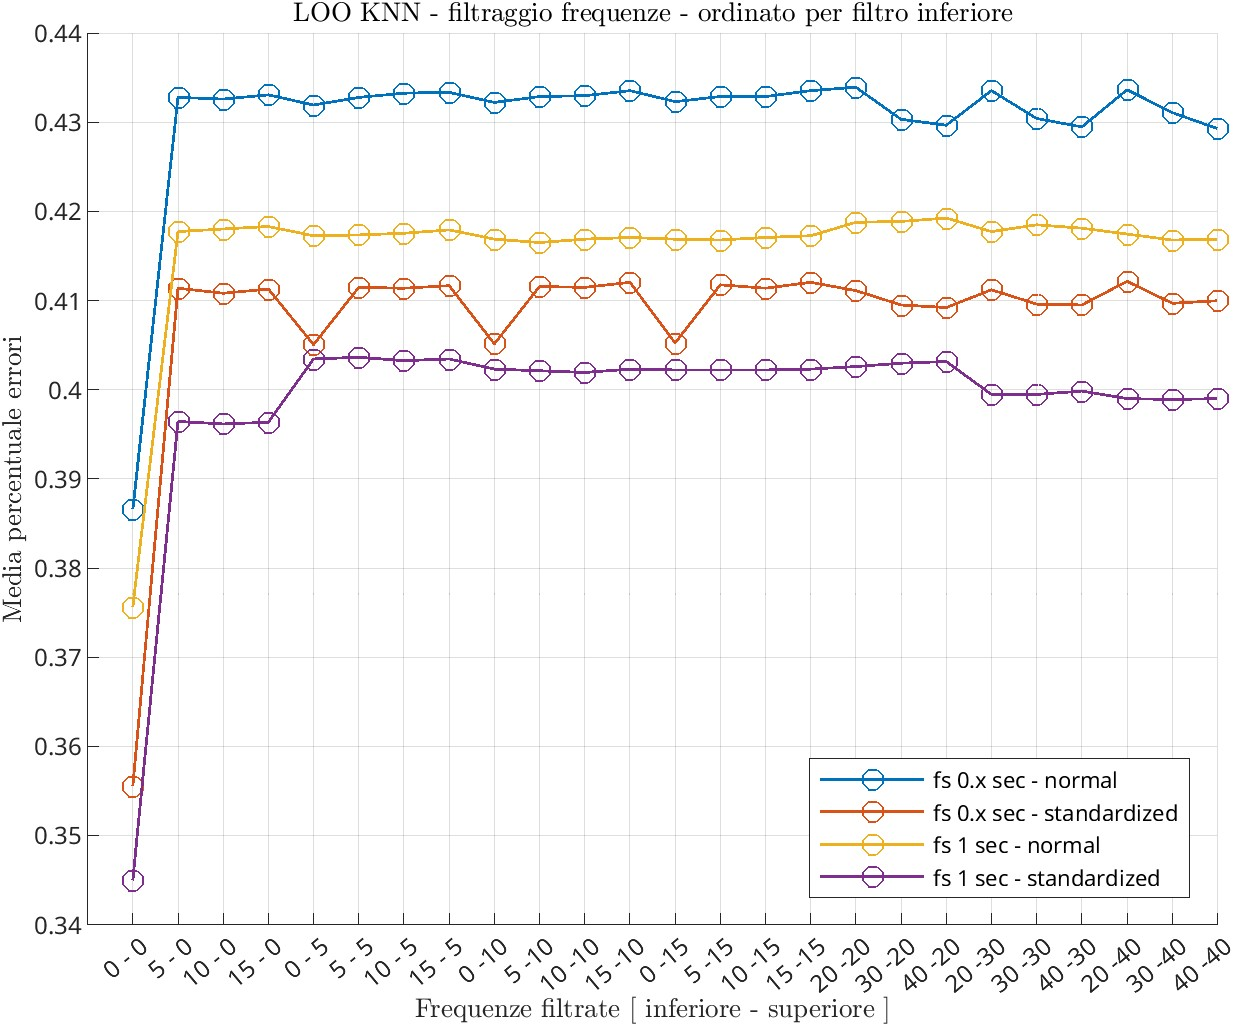
\includegraphics[width=1\textwidth]{img/cap4-filtraggio1.jpg}
		\caption{Risultato filtraggio frequenze ordinato per filtro inferiore. Sull'asse dell'ordinate è esposta la media dell'errore ottenuto per ogni combinazione di filtri presenti sull'asse delle ascisse.}
		\label{fig4.1}
	\end{figure}
\end{center}	
\begin{center}	
	\begin{figure}[htp]
		\centering
		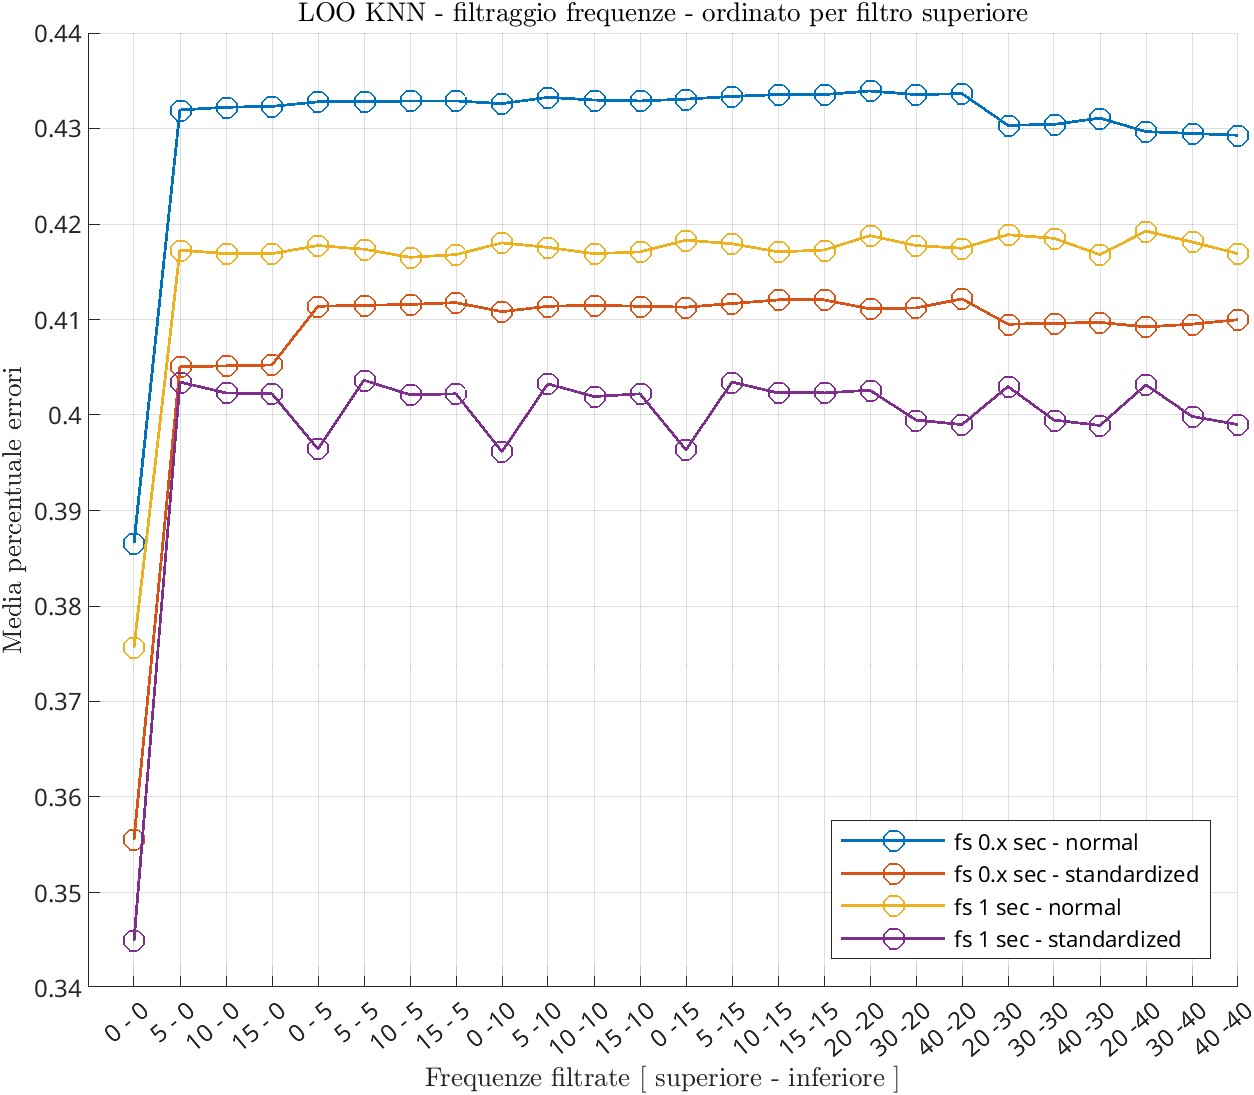
\includegraphics[width=1\textwidth]{img/cap4-filtraggio2.jpg}
		\caption{Risultato filtraggio frequenze ordinato per filtro superiore. Sull'asse dell'ordinate è esposta la media dell'errore ottenuto per ogni combinazione di filtri presenti sull'asse delle ascisse.}
		\label{fig4.2}
	\end{figure}
\end{center}	

\clearpage
\subsection{Risultati problemi con etichette oggettive}
In questa sezione si riportano i risultati della prima analisi di classificazione, basata su
rappresentazione tramite categorie oggettive.

Nel grafico della figura 4.3 si può visualizzare l’esito dei casi sottoposti: sull’asse delle ordinate troviamo
l’errore medio ottenuto dal classificatore, su quello delle ascisse il tipo di problema. Le barre
colorate su ogni problema rappresentano le quattro finestre temporali considerate:
FS0X.NOR, FS1.NOR, FS0X.STD, FS1.STD.

Il miglior risultato lo si individua nel caso PR-1.1 YAT, il problema che che ha come
obiettivo di individuare il luogo di registrazione, gli \textit{yat}. Nella configurazione migliore si
ottiene un errore del 0.9\%. Questo problema è l’unico tra quelli con categorie oggettive che
tratta della discriminazione del luogo. Sicuramente ha goduto, oltre alle peculiarità della zona
in sé, persino delle caratteristiche dello stato dello strumento di misurazione. Si può
ipotizzare che elementi come le interferenze o le condizioni meteorologiche, colpendo
indifferentemente i vari sensori, abbiano marchiato il prodotto segnando maggiormente uno
tra questi rispetto agli altri per un determinato periodo temporale: hanno caratterizzato una
parte del registrato e contribuito ad accrescere le già notabili differenze, definite
dall’ambiente circostante, con il resto dei dispositivi. Non di meno, un altro dettaglio
importante riguarda il suono rappresentante dell’elemento cascata C, che è quasi
onnipresente, poiché lo si ritrova nella totalità delle registrazioni, ma in versioni eterogenee
tra i dispositivi, dato che sono posizionati a distanze differenti dalla sorgente del rumore. E’
possibile affermare che una discriminazione basata sul luogo ha sicuramente beneficiato di
queste condizioni rispetto alle altre casistiche.

D’altra parte, anche le tipologie sviluppate sulla temporalità hanno ottenuto complessivamente 
dei buoni risultati. L’idea alla base dei casi PR-1.2 G/N e PR-1.3 AT/R di
caratterizzare i periodi astronomici dell’alba e del tramonto, ha portato delle conclusioni
interessanti, in particolare nel secondo, che si basava proprio sul discriminare questi due
momenti principali rispetto al resto della giornata. Nelle migliori configurazioni si è ottenuto
un errore del 14\% per PR-1.2 G/N e del 25\% per PR-1.3 AT/R. Pur sapendo che in un
contesto naturale presentano delle caratteristiche sonore uniche, si rende noto, che,
diversamente dalle aspettative, il sistema di classificazione non è stato così efficace per il
problema PR-1.4 A/T/G/N, risultato con la maggiore percentuale di errori in una media del
50\%. Ovviamente c’è il numero delle classi (4) superiore rispetto agli altri scenari, portando
una notevole complessità quindi una minore capacità di generalizzazione. Inoltre, è possibile
ipotizzare che il risultato sia stato determinato anche dalla riduzione della quantità dei dati di
addestramento da cui estrarre un modello identificativo di ogni classe: avendo un numero
finito di campioni all’aumentare della classi diminuisce il numero di oggetti per descriverle.
Per quanto riguarda le finestre considerate, si evidenzia dal grafico, mediante i colori delle
barre, come la FS1.STD (finestra minore di un secondo normalizzata) abbia ottenuto le
migliori prestazioni in ogni problema di classificazione. Si può ipotizzare che la finestra più
ampia permetta di cogliere maggiori dettagli di interesse nel contesto: una finestra con
maggiore risoluzione potrebbe risultare vantaggiosa per lo studio. A tale risoluzione anche il
rumore potrebbe risultare meno influente, non facendo quindi risaltare determinati elementi
irrilevanti per la classificazione. Allo stesso modo, anche l’altra versione standardizzata
FS0X.STD ha riportato un esito accettabile e abbastanza simile alla finestra appena descritta.
Se consideriamo l’effetto della standardizzazione, possiamo osservare come entrambe le
versioni standardizzate hanno conseguito un errore minore rispetto alle controparti regolari.
Si considera però che, la finestra più corta, ma con dati standardizzati, FS0X.STD, nella
maggioranza dei casi ha ottenuto dei risultati migliori della finestra più ampia ma con dati
normali, FS1S.NOR. Quindi si può dedurre che per il contesto la scelta corretta sia una
combinazione tra la finestra più ampia e dati standardizzati.

Il grafico in figura 4.4 mostra la medesima situazione sotto un'altra prospettiva cioè dal punto di vista
delle \textit{features}, sintetizzando per ogni configurazione il suo errore medio tra i vari problemi
disegnati. Nei gruppi con le features singole ORIG gli errori per tipologia di finestra si
discostano di poco, diversamente che nelle forme combinate dove le versioni standardizzate
sono maggiormente incisive. Lo si può notare nel gruppo CONC.MED.ORIG., che ottiene i
migliori risultati in entrambe le versioni standardizzate con un errore medio intorno al 18\%.
Riassume le caratteristiche essenziali dei tre gruppi SPE/TON/TEM, servendosi di un numero
ristretto di \textit{features}, undici in questo caso. Un insieme di componenti ridotto, riduce la
complessità del modello, rendendolo più robusto, aumentando la sua interpretabilità e
ottenendo una migliore generalizzazione.

\begin{center}	
	\begin{figure}[htp]
		\centering
		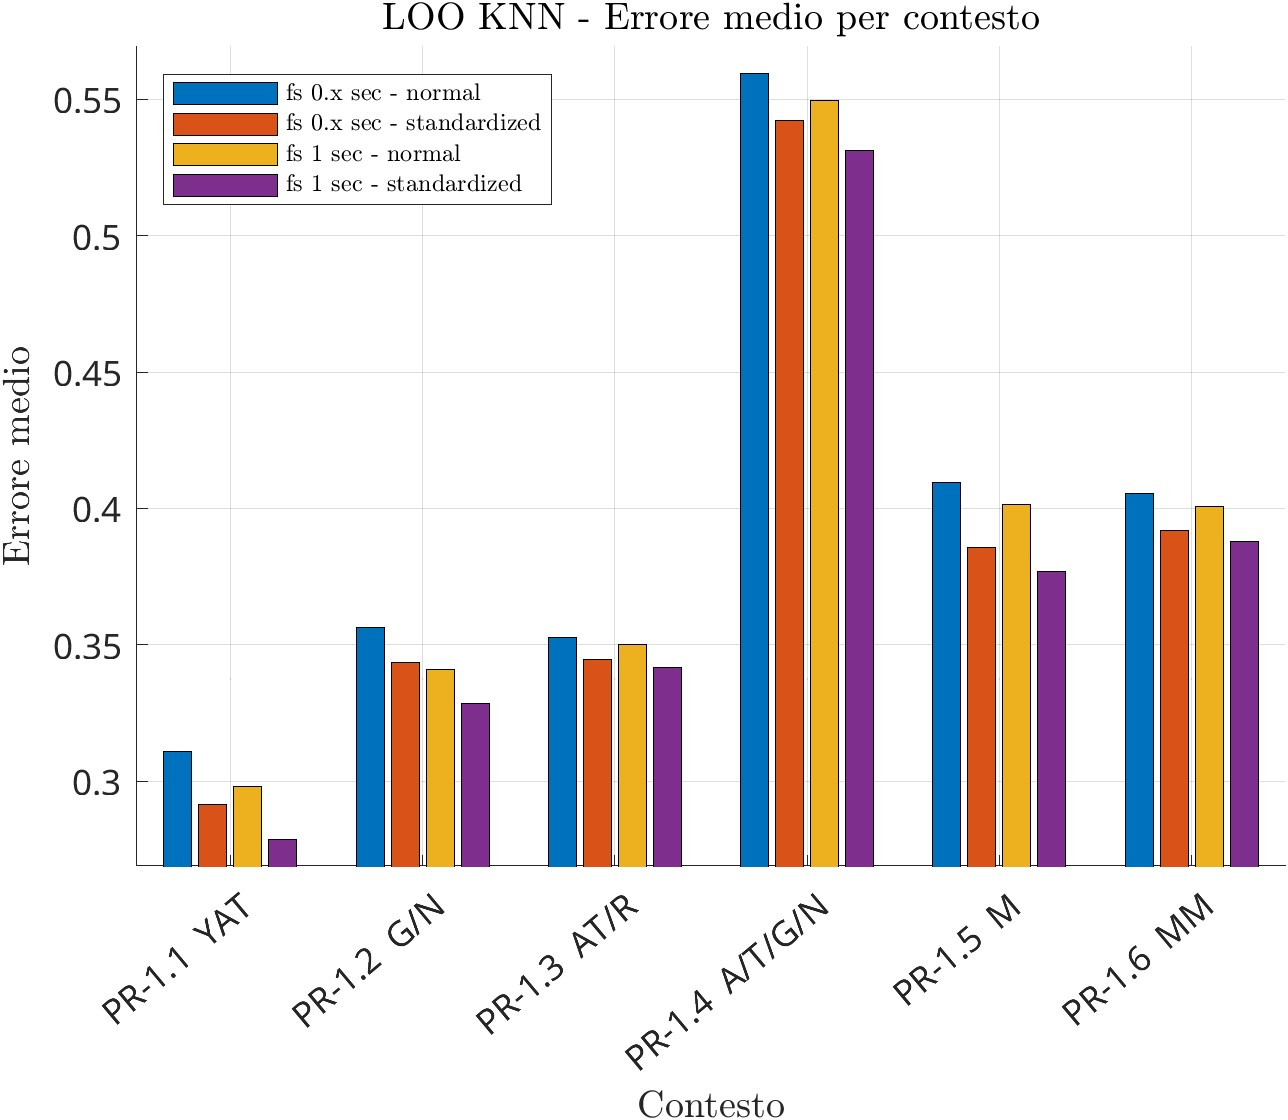
\includegraphics[width=1\textwidth]{img/cap4-classificazione_fase1_binaria.jpg}
		\caption{Errore medio nei problemi di classificazione disegnati per le quattro finestre temporali considerate.}
		\label{fig4.3}
	\end{figure}
\end{center}	
\begin{center}	
	\begin{figure}[htp]
		\centering
		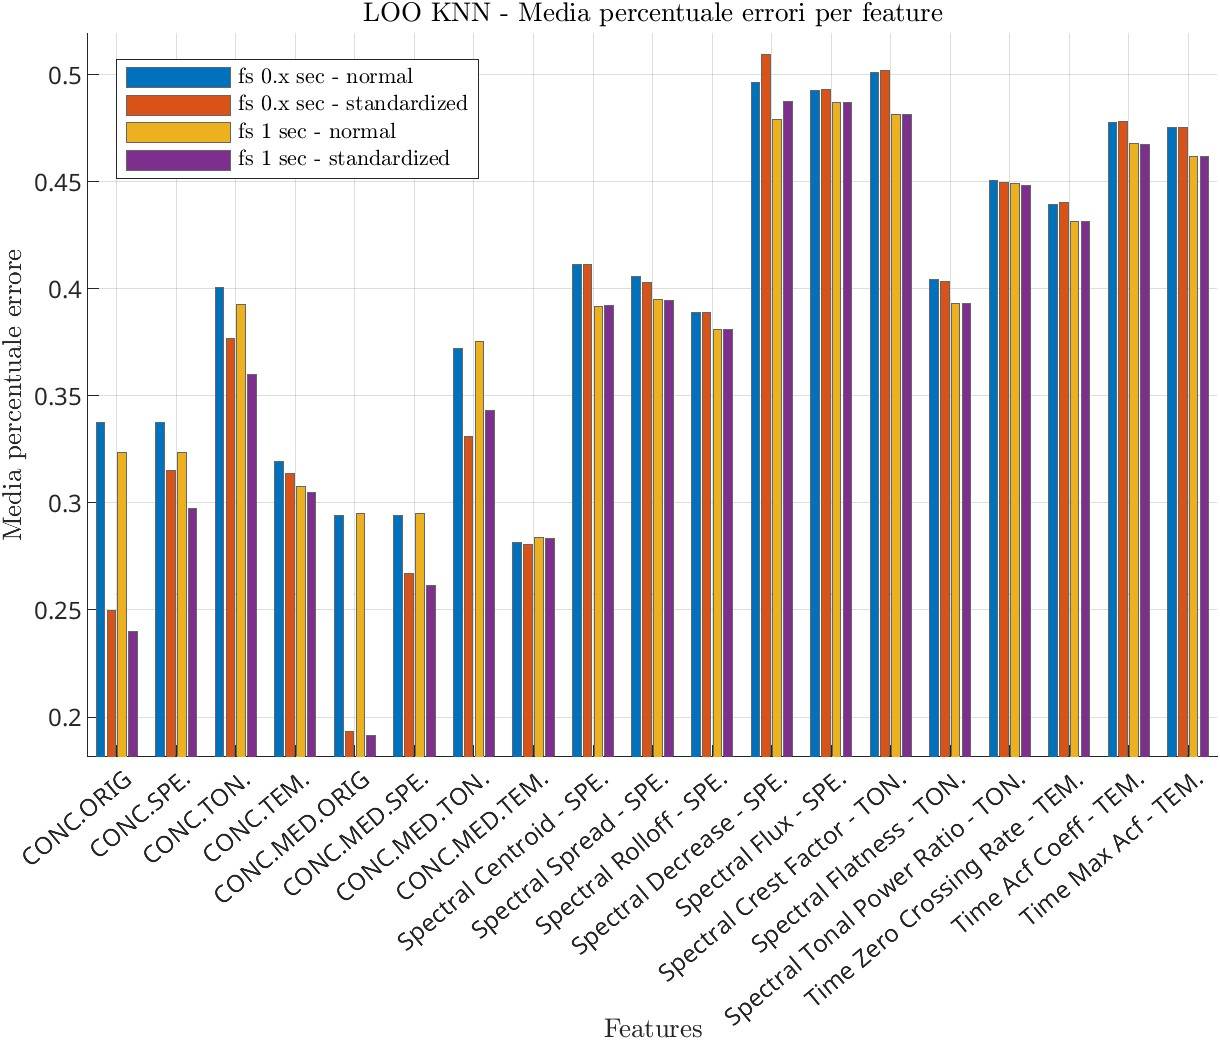
\includegraphics[width=1\textwidth]{img/cap4-classificazione_fase1_features.jpg}
		\caption{Errore medio dei problemi di classificazione dal punto di vista delle features per le quattro finestre.}
		\label{fig4.4}
	\end{figure}
\end{center}

\cleardoublepage
\subsection{Risultati problemi con etichette semantiche}
Nel corrente paragrafo andremo ad analizzare i risultati della seconda fase di classificazione
che analizza i problemi rappresentati da categorie semantiche. Come precedentemente
affermato, tali casistiche sono state disegnate in una condizione multi-etichetta, ovvero che
ogni audio è caratterizzato da più suoni, quindi più etichette assegnate allo stesso oggetto.

In generale possiamo sostenere che gli esperimenti con la versione standardizzata ottengono
una media di errore minore rispetto alla controparte non normalizzata, nel dettaglio, la
versione FS1.STD primeggia costantemente. Lo si può osservare nel grafico in figura 4.5 che riassume
gli esiti dei problemi disegnati, sintetizzando per ogni configurazione il suo errore medio tra i
vari problemi disegnati. È chiaro che il valore medio in queste analisi permette di trarre una
visione generale dell’insieme. Tuttavia, si sottolinea che a causa dello scarso risultato di
alcune \textit{features}, l’esito può essere sbilanciato. Per questo verranno comunque evidenziati i
dati che spiccano rispetto al gruppo, ma che potrebbero discostarsi in alcuni casi dai quelli
esposti nel grafico. Si evidenzia che, siccome nel grafico i casi di classificazione a tre classi
hanno avuto un errore fuori scala rispetto alla media generale, si è deciso per comprimere una
parte dell’asse delle ordinate per ottenere una migliore visione dell’insieme: la zona
compressa riguarda i valori tra 0.44 e 0.54 evidenziata sul grafico mediante una barra
orizzontale grigia, la fascia intermedia presente tra i risultati a due e tre classi.
A seguire saranno descritti nel dettaglio i tre gruppi elencati nel paragrafo 4.4.2.

In merito ai casi di classificazione PR-2.1 (binari) che discriminano la presenza/assenza di
una determinata classe, i risultati mostrano un errore medio nei problemi disegnati intorno al
39\% di errore. È possibile notare che la classe V ottiene un lieve miglioramento con la
finestra FS0X.NOR, diversamente dagli altri casi, dove invece vediamo sempre prevalere la
versione FS1.STD.

In questo gruppo i problemi con i migliori risultati riguardano i suoni appartenenti alla GEO,
delle classi T e P nei problemi PR-2.1.3 P con il 24\% di errore e PR-2.1.4 T con il 26\%. Si
evidenzia il risultato delle feature CONC.MED.SPE, che primeggia in entrambe le frequenze,
con una media di errori pari al 33\%, e in un posizione molto vicina anche la feature
CONC.MED.ORIG. Il loro risultato lo si può notare nel grafico in figura 4.6, che mette in evidenza il
comportamento delle features trasversalmente ai casi sottoposti, con una media sui valori. È
possibile notare che anche CONC.SPE. e CONC.ORIG, hanno ottenuto in generale un buon
risultato. In questo gruppo la BIO sembra essere stata caratterizzata dalle \textit{features} spettrali.

Per quanto concerne il gruppo PR-2.2, classificazione binaria ma con due classi distinte i
risultati sono soddisfacenti per il nostro contesto con una media di errore del 39\%.
Probabilmente anche perché le classi sono più bilanciate. Questi problemi hanno permesso di
valutare gli insiemi ANT/BIO/GEO in contrapposizione a coppie, evidenziando delle
differenze rilevanti. È possibile notare l’ANT in contrasto con la GEO, nel problema
PR-2.2.1 V/P con una media di errore del 43\%, dove si ottengono risultati peggiori rispetto al
confronto con la BIO, nel problema PR-2.2.2 V/G con una media di errore del 38\%: è
ipotizzabile supporre che il suono dei grilli, essendo discontinuo come il suono del veicolo,
ha permesso al sistema di poterli discriminare più facilmente, a differenza invece, del suono
della pioggia, che si mantiene persistente. Allo stesso modo, lo ritroviamo nella correlazione
di BIO con ANT, in PR-2.2.1 V/P con una media di errore del 43\%, e BIO con GEO, in
PR-2.2.4 G/P con una media di errore del 37\%: si nota nel primo una maggiore difficoltà,
come appena evidenziato. La minima presenza del suono di veicoli all’interno del dato ha
sicuramente influito sul modello, quindi è possibile ipotizzare che il suono dei grilli con la
pioggia abbia permesso un confronto simile al suono del veicolo con la pioggia, essendo
entrambi molto percepibili. Differentemente, potendo valutare due casi relativi allo stesso
confronto BIO/GEO, in PR-2.2.3 G/T e PR-2.2.4 G/P, è osservabile un comportamento
simile, con valori leggermente migliori dei casi sopra esposti, con un media di errore del 37\%
e nelle configurazioni migliori un errore del 20\%. Si ipotizza che l’origine simile, per T e P,
pur essendo suoni diversi, converga in un intervallo di frequenze simili, che rispecchiano la
GEO. Da un punto di vista delle features, si evidenzia che, in maniera simile al primo gruppo
i risultati migliori sono dati dalla versione standardizzata per CONC.ORIG e CONC.SPE per
quanto riguarda il problema PR-2.2.4 G/P, con un 20\% medio di errore. Invece con un 25\%
negli altri casi per le stesse versioni ma con le medie concatenate in CONC.MED.ORIG e
CONC.MED.SPE.. Tali valori si possono notare nel grafico in figura 4.6, che espone i risultati dalla
prospettiva delle \textit{features}.

Nei casi di classificazione a tre classi, PR-2.3.1 V/G/P e PR-2.3.2 V/G/T, i risultati si sono
rivelati inferiori alle aspettative con un errore medio di circa del 54\%. Le classi pur essendo
bilanciate, si trovavano in quantità significativamente minori. Inoltre, il numero di classi, pari
a tre, ha complicato ulteriormente il modello, unitamente ai possibili disturbi causati dagli
altri suoni non inerenti al problema. Dal punto di vista delle features invece si nota un
comportamento diverso dai casi precedenti. Infatti, nel primo caso PR-2.3.1 V/G/P otteniamo
i migliori risultati con le \textit{feature} CONC.MED.ORIG, nella versione standardizzata in
particolare, invece nel secondo caso PR-2.3.2 V/G/T, vediamo protagonista la CONC.MED.TON 
con un errore del 40\% circa, per entrambe le finestre ed entrambe le forme
normali e standardizzate. Il grafico in figura 4.8 ci propone i dati del gruppo dal punto di vista delle
\textit{features}.

È possibile presupporre che ogni risultato sia stato influenzato negativamente dalla presenza
di altri suoni non considerati nel problema in esame, come, allo stesso tempo, la quantità
limitata di dati a disposizione per classe potrebbe conseguire un scarso addestramento
condizionando la capacità di generalizzazione del discriminatore.

In sintesi, possiamo evidenziare che i tutti i casi analizzati le feature CONC.MED.ORIG si
dimostrano tra le migliori per descrivere i vari casi esposti, seguite da CONC.MED.SPE. nel
particolare dei casi binari, e da CONC.MED.TON. per i casi ternari. In particolare,
esprimono al meglio il loro potenziale nella versione con la finestra FS1.STD, che è risultata
superiore nella maggioranza delle casistiche.

\vspace{12pt}

\begin{center}	
	\begin{figure}[htp]
		\centering
		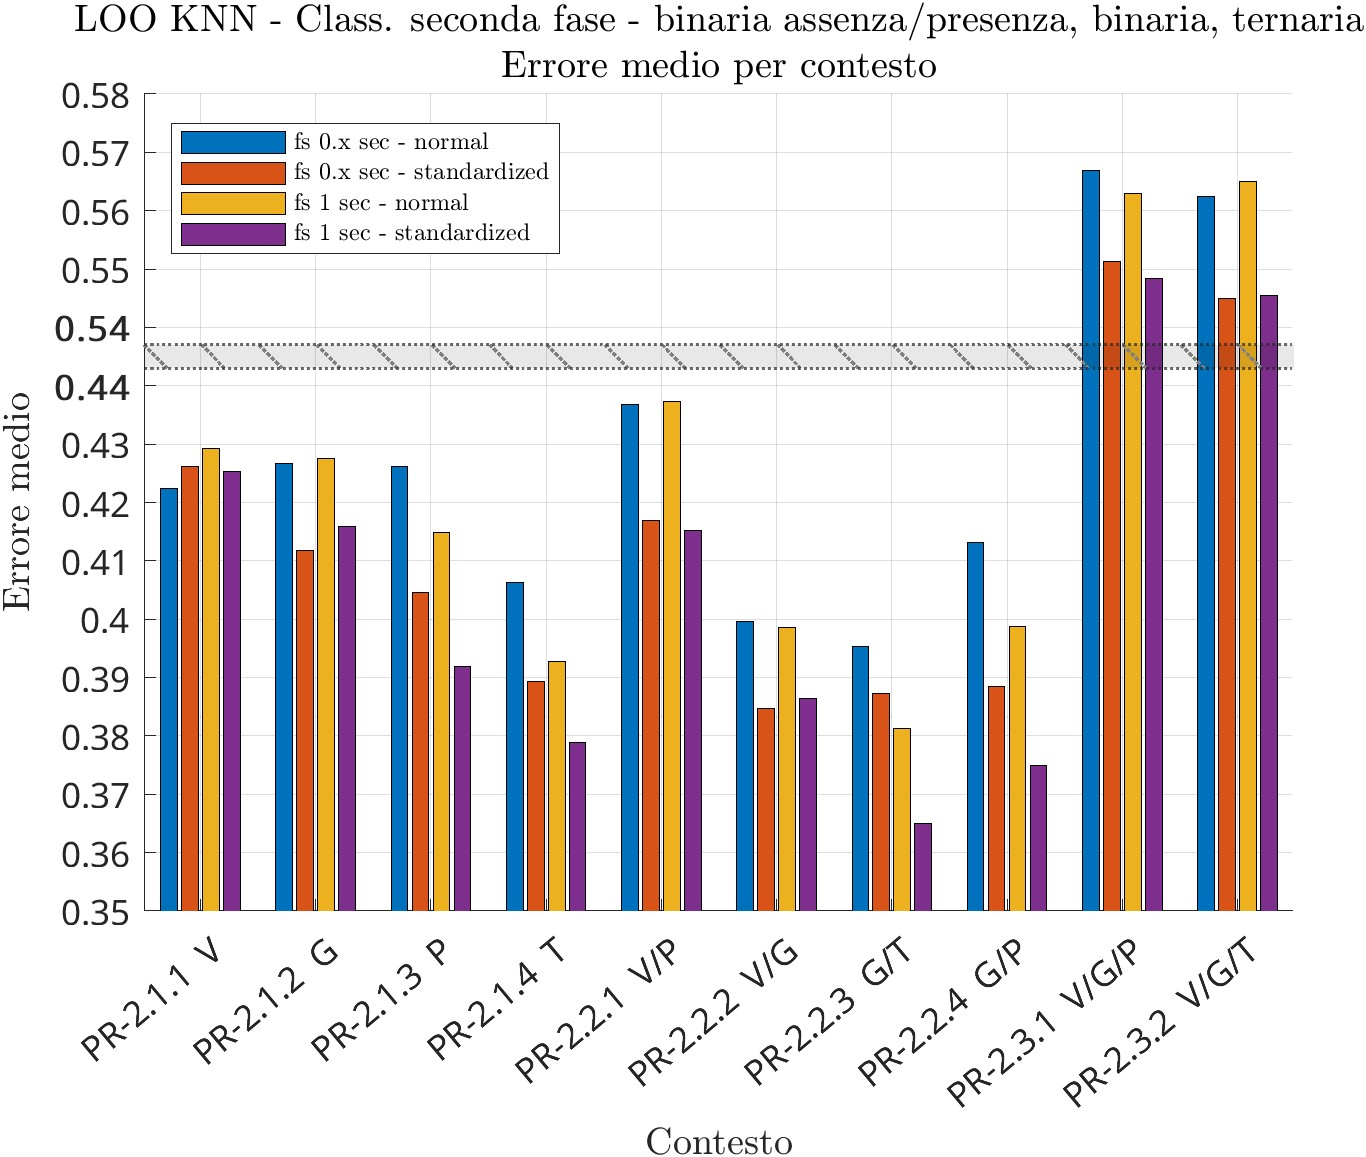
\includegraphics[width=0.9\textwidth]{img/cap4-classificazione_fase2_problemi.jpg}
		\caption{Risultati problemi di classificazione con categorie semantiche. Le barre colorate identificano per
			ogni problema le quattro finestre impiegate. Il risultato esposto è la sintesi dell’errore medio ottenuto con tutte
			le configurazioni di features. La barra grigia orizzontale indica una zona in cui i dati sono stati compressi per
			ottenere una migliore visione del grafico.}
		\label{fig4.5}
	\end{figure}
\end{center}	
\begin{center}	
	\begin{figure}[htp]
		\centering
		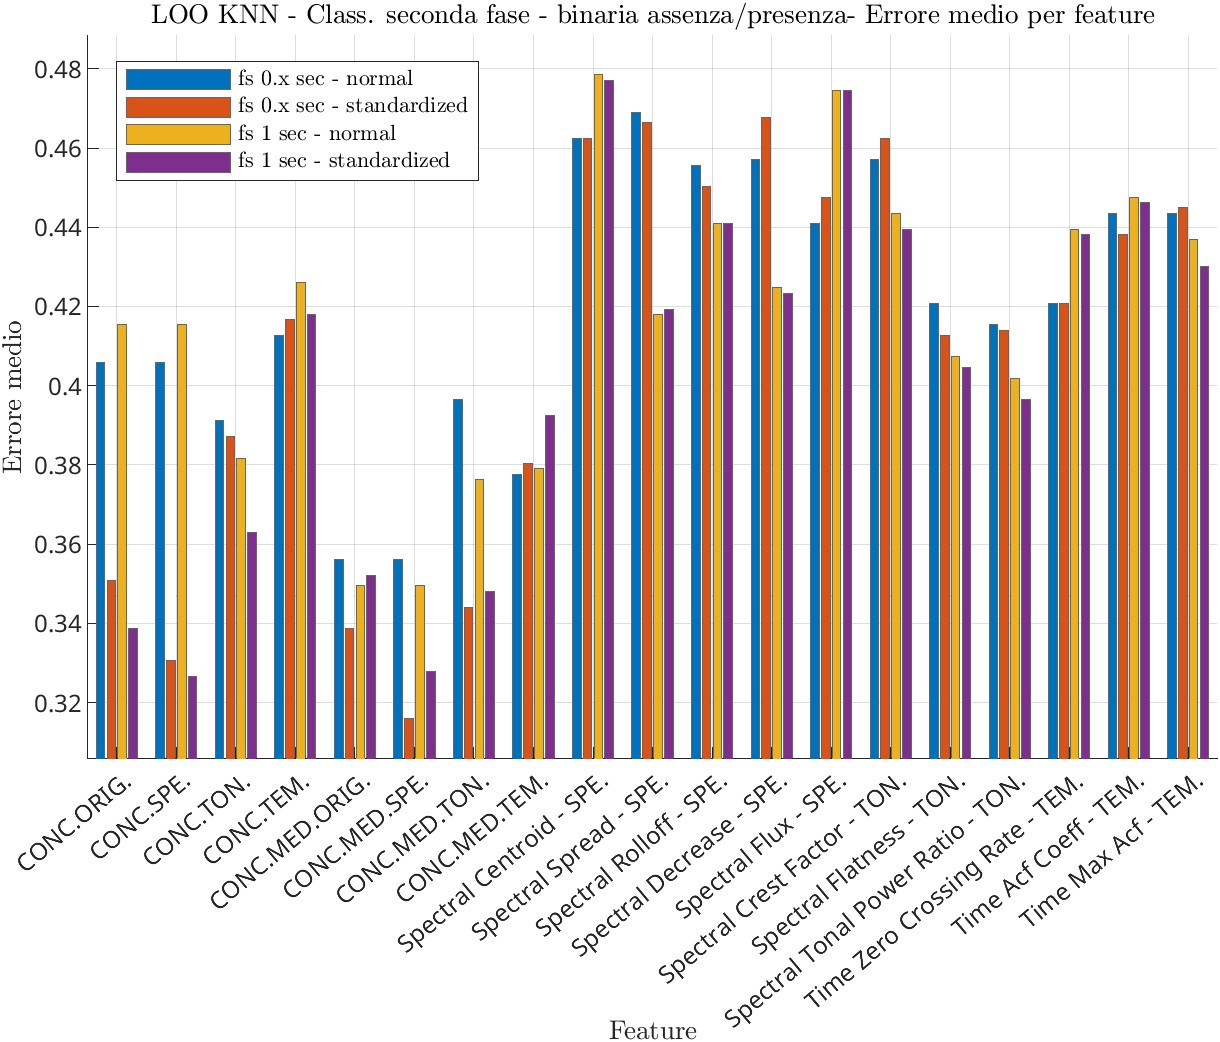
\includegraphics[width=1\textwidth]{img/cap4-classificazione_fase2_features_binaria_presenza.jpg}
		\caption{Risultati problemi di classificazione binaria presenza/assenza con categorie semantiche dal punto
			di vista delle \textit{features}. Le barre colorate identificano per ogni \textit{features} le quattro finestre impiegate. Il risultato
			esposto è la sintesi dell’errore medio tra i vari problemi disegnati.}
		\label{fig4.6}
	\end{figure}
\end{center}
\begin{center}	
	\begin{figure}[htp]
		\centering
		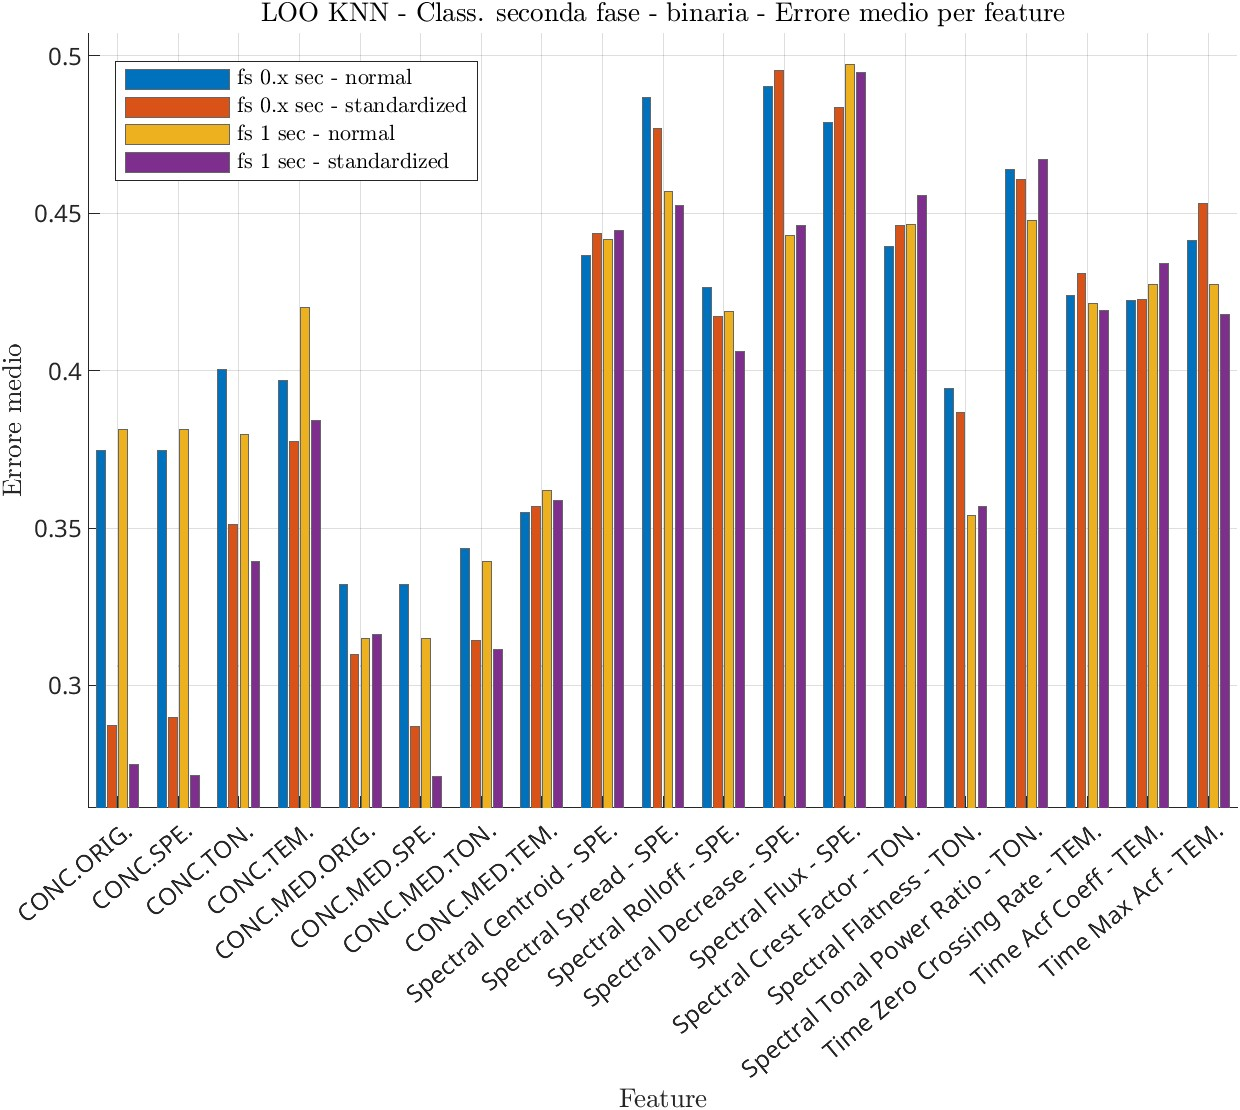
\includegraphics[width=1\textwidth]{img/cap4-classificazione_fase2_features_binaria_distinte.jpg}
		\caption{Risultati problemi di classificazione binaria a due classi distinte con categorie semantiche dal punto di
			vista delle \textit{features}. Le barre colorate identificano per ogni \textit{features} le quattro finestre impiegate. Il risultato
			esposto è la sintesi dell’errore medio tra i vari problemi disegnati.}
		\label{fig4.7}
	\end{figure}
\end{center}	
\begin{center}	
	\begin{figure}[htp]
		\centering
		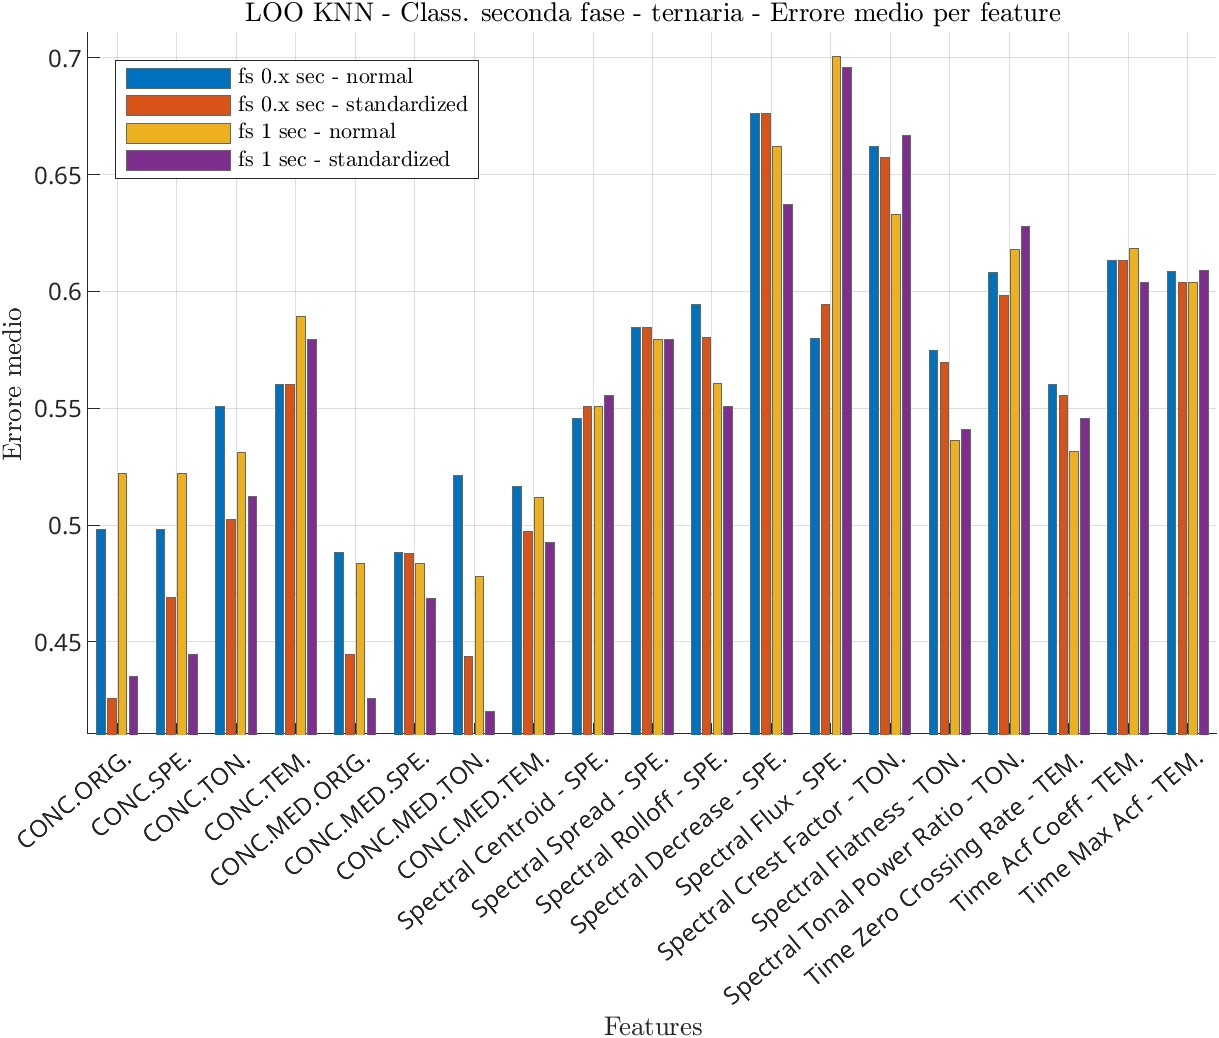
\includegraphics[width=1\textwidth]{img/cap4-classificazione_fase2_features_ternaria.jpg}
		\caption{Risultati problemi di classificazione a tre classi con categorie semantiche dal punto di
			vista delle \textit{features}. Le barre colorate identificano per ogni \textit{features} le quattro finestre impiegate. Il risultato esposto è la sintesi dell’errore medio tra i vari problemi disegnati.}
		\label{fig4.8}
	\end{figure}
\end{center}

	\clearpage\cleardoublepage\chapter{Anomaly Detection}
In questo capitolo si andrà ad esporre la terza fase dello studio, che si occupa di studiare
algoritmi di A.D. per individuare eventuali suoni anomali. Nel contesto dei \textit{soundscape} gioca
un ruolo molto interessante, per identificare suoni o eventi insoliti che potrebbero indicare
cambiamenti ambientali, rumori estranei o fenomeni singolari: per esempio, la presenza di un
cacciatore, oppure un animale non appartenente alla fauna del luogo. In questa analisi si è
deciso di sperimentare l’utilizzo di tale metodologia applicando le conoscenze ottenute dalle
fasi precedenti, per inferire informazioni ed esaminare quali elementi vengono classificati
come anomali.

\section{Configurazione \textit{features} e metodi}
Nel seguente paragrafo saranno descritte le \textit{features} utilizzate in questo studio e le
configurazioni dei metodi esposti nel paragrafo 2.3. Come menzionato sopra, la conoscenza
ottenuta con lo studio di classificazione ci ha permesso di individuare \textit{feature} che riescono ad
caratterizzare chiaramente il \textit{dataset}. Inoltre, dai risultati si è potuto verificare quale delle due
finestre sia in grado di definire le caratteristiche più rilevanti. Si è quindi utilizzato il set di
feature della versione FS1 di entrambe le forme di dati, per un totale di 38 \textit{features}, 19
normali (FS1.NOR) e 19 standardizzate (FS1.STD).

Per quanto riguarda i metodi, le versioni utilizzate presentano delle configurazioni
considerabili come standard, quindi non sono state fatte particolari ottimizzazioni. IF utilizza
100 alberi decisionali, un valore largamente utilizzato; la scelta di un numero maggiore
potrebbe determinare una maggiore robustezza del modello, ma incrementa notevolmente
anche il tempo di calcolo. Il numero di campionamenti presi per ogni albero è di 256
elementi. Per LOF, invece, si è fissato per k (vicini) il valore di venti elementi, e come
metrica di distanza, quella euclidea, già descritta precedentemente. Per l’algoritmo OCSVM,
infine, si è utilizzato il kernel gaussiano. Il fattore di contaminazione, ovvero la soglia
decisionale per definire quali elementi trattare come anomalie, è stato impostato a zero per
tutti e tre gli algoritmi. Con tale valore il sistema non avendo una soglia definita per capire se
un elemento è un'anomalia o meno, tratta tutti gli elementi come normali, assegnandogli solo
un punteggio di anormalità. Si è deciso di non considerare il fattore di contaminazione dato
che, nell’ambito dello studio è molto difficile definire una soglia a priori che possa definire l'anormalità. 
Si è deciso di valutare invece gli elementi che con maggior frequenza risultano tra i punteggi più alti dei risultati delle
configurazioni di \textit{features}.

\section{Validazione dei risultati}
In questo paragrafo verrà descritta la modalità di validazione per le tecniche A.D. nel
contesto dello studio. Gli algoritmi sopra descritti fanno parte della tipologia di approcci non
supervisionati, ovvero non necessitano quindi di etichette per poter funzionare. Per avere la
validazione, è stato comunque impiegato il dataset DATA2, che è etichettato, così da potersi
servire delle conoscenze sul contenuto per verificare il risultato.

Le modalità di analisi prevedono trenta esecuzioni dell’algoritmo, calcolando la media dei
punteggi di anomalia, in maniera tale da essere indipendenti dal valore della singola
esecuzione. L’approccio viene replicato per ciascuna \textit{feature} (38, 19 normali e 19
standardizzate), considerando poi solo i tre risultati con punteggio maggiore per feature,
ottenendo un insieme totale di 38 x 3 risultati per ogni metodo. Per la valutazione del metodo
sono state estratte le prime cinque occorrenze più numerose dai risultati del metodo. Per avere visione complessiva,
invece, sono state estratte le prime cinque occorrenze più numerose considerando tutti e tre
gli insiemi di risultati.

\section{Risultati}
Dopo aver esposto la modalità di applicazione dell’analisi si andrà a descrivere i risultati
ottenuti. Nella tabella in figura 5.1 è possibile avere una visione dei risultati come descritti nel
paragrafo precedente. I dati sono divisi in quattro gruppi definiti dalla prima colonna: i primi
tre riguardano i risultati dei singoli metodi applicati ovvero IF, LOF e O, e il quarto i risultati
sul totale. Per ognuno gruppo vengono esposti i primi cinque oggetti che hanno ottenuto più
occorrenze. Nella seconda colonna si ha la descrizione dell’oggetto riscontrato come
anomalia e nella terza colonna il numero di occorrenze rilevate all'interno del gruppo che identificano il file come anomalo. Nelle restanti colonne sono elencati i suoni presenti all’interno dell’audio riscontrato come
anomalia. Per ogni gruppo viene indicato il relativo risultato percentuale della presenza sonora di un determinato suono all'interno del gruppo.

Dal punto di vista dei singoli suoni, gli oggetti più anomali presentano: il rumore dei veicoli
rilevato per un 40\% su IF e O, per un 60\% invece per L; il suono degli uccelli U che è sempre
presente per un 60\% e con una distribuzione simile in tutte e tre le casistiche; il suono dei
grilli G, che è emerso presente per un 40\% e solo in L; il suono del fiume/cascata C, che,
come prevedibile, appare molto diffuso tra i risultati, ma si può ipotizzare che non abbia nulla
di particolare e che la sua presenza sia dovuta unicamente alla sua ampia distribuzione nei
dati; il suono della pioggia P che si è notevolmente osservato, per un 80\%, e si può affermare
che valgono le stesse conclusione appena fatte per il caso precedente; infine, le interferenze e
i suoni sconosciuti non sono stati rilevati come anomalie, contrariamente alle aspettative. Ci
si poteva aspettare che sarebbero emersi data la loro minima presenza e particolarità, ma
invece sono stati rilevati solo per un caso, e solo dal metodo O.

Come è possibile notare, dalla prospettiva dei metodi, si vede che IF e O hanno espresso delle
distribuzioni simili negli oggetti anomali rilevati nella BIO con il suono degli uccelli U per un
60\% e nessun caso che contenesse dei grilli G, nella GEO con il suono di cascata C e pioggia
P per un 80\% e infine nessuna presenza di interferenza. Invece, il metodo L ha dimostrato
una sensibilità diversa, maggiore per il suono della cascata C, rilevata nel 100\% degli oggetti
anomali, e una minore invece per la pioggia P per un 40\%.

Invece, se si osserva dal punto di vista degli insiemi di suoni ANT/BIO/GEO, si può notare
come la GEO sia molto presente, per almeno un 80\%. Per una parte si possono trarre le stesse
conclusioni definite prima sulla distribuzione dei suoni C e P, ma per quanto riguarda quello
di T, si può ipotizzare che non lo sia. Infatti, la sua distribuzione nel dataset di riferimento è
di circa del 60\%, e la sua bilanciata presenza tra i risultati si può ritenere molto interessante.
Similmente, per ANT e BIO è possibile sostenere l’ipotesi che il risultato ottenuto sia
rilevante: per il primo sulla bassa numerosità dei dati in input, per il secondo invece, data la
sua grande distribuzione, perché non si è propagato similmente a quanto osservato nei suoni
più rilevati della GEO.

Infine, da una prospettiva temporale, si manifesta che l’80\% dei risultati sul totale, ma anche
nei singoli algoritmi, si concentra alle ore 14:00, nella seconda parte della giornata. Lo stesso
per l’elemento identificato maggiormente come anomalia che risulta invece verso le ore
18:00.

%\begin{table}[ht]
%	\centering
%	\begin{tabular}{@{}lclcccccccc@{}}
%		\toprule
%		& \multicolumn{1}{l}{} &  & \multicolumn{1}{l}{\cellcolor[HTML]{FCEFEE}\textbf{ANT.}} & \multicolumn{2}{c}{\cellcolor[HTML]{9FE887}{\color[HTML]{000000} \textbf{BIO.}}} & \multicolumn{3}{c}{\cellcolor[HTML]{B0E4F3}\textbf{GEO.}} & \multicolumn{2}{c}{\cellcolor[HTML]{FFFFFF}\textbf{ALTRO}} \\ \cmidrule(l){4-11} 
%		\textbf{Gruppo} & \multicolumn{1}{c}{\textbf{\# occ.}} & \multicolumn{1}{c}{\textbf{Audio}} & \textbf{V} & \textbf{U} & \textbf{G} & \textbf{C} & \textbf{P} & \textbf{F} & \textbf{I} & \textbf{S} \\ \midrule
%		& 22 & 20200323\_180000.WAV & x & x &  & x & x &  &  &  \\
%		& 18 & 20200303\_140000.WAV &  &  &  &  & x & x &  &  \\
%		& 12 & 20200304\_140000.WAV &  &  &  & x & x & x &  &  \\
%		& 8 & 20200309\_060000.WAV & x & x &  & x &  &  &  &  \\
%		& 8 & 20200316\_220000.WAV &  & x &  & x & x &  &  &  \\ \cmidrule(l){2-11} 
%		\multirow{-6}{*}{\textbf{IF}} & \multicolumn{2}{c}{\cellcolor[HTML]{EFEFEF}\textbf{RISULTATO \%}} & \cellcolor[HTML]{EFEFEF}\textbf{40} & \cellcolor[HTML]{EFEFEF}\textbf{60} & \cellcolor[HTML]{EFEFEF}\textbf{0} & \cellcolor[HTML]{EFEFEF}\textbf{80} & \cellcolor[HTML]{EFEFEF}\textbf{80} & \cellcolor[HTML]{EFEFEF}\textbf{40} & \cellcolor[HTML]{EFEFEF}\textbf{0} & \cellcolor[HTML]{EFEFEF}\textbf{0} \\ \midrule
%		& 15 & 20200311\_140000.WAV &  &  &  & x & x & x &  &  \\
%		& 15 & 20200323\_180000.WAV & x & x &  & x & x &  &  &  \\
%		& 10 & 20200318\_140000.WAV & x & x &  & x &  &  &  &  \\
%		& 9 & 20200301\_180000.WAV &  & x & x & x &  & x &  &  \\
%		& 8 & 20200325\_020000.WAV & x &  & x & x &  &  &  &  \\ \cmidrule(l){2-11} 
%		\multirow{-6}{*}{\textbf{LOF}} & \multicolumn{2}{c}{\cellcolor[HTML]{EFEFEF}\textbf{RISULTATO \%}} & \cellcolor[HTML]{EFEFEF}{\color[HTML]{000000} \textbf{60}} & \cellcolor[HTML]{EFEFEF}{\color[HTML]{000000} \textbf{60}} & \cellcolor[HTML]{EFEFEF}{\color[HTML]{000000} \textbf{40}} & \cellcolor[HTML]{EFEFEF}{\color[HTML]{000000} \textbf{100}} & \cellcolor[HTML]{EFEFEF}{\color[HTML]{000000} \textbf{40}} & \cellcolor[HTML]{EFEFEF}{\color[HTML]{000000} \textbf{40}} & \cellcolor[HTML]{EFEFEF}{\color[HTML]{000000} \textbf{0}} & \cellcolor[HTML]{EFEFEF}{\color[HTML]{000000} \textbf{0}} \\ \midrule
%		& 6 & 20200323\_180000.WAV & x & x &  & x & x &  &  &  \\
%		& 5 & 20200309\_060000.WAV & x & x &  & x &  &  &  &  \\
%		& 4 & 20200314\_180000.WAV & x & x &  & x & x & x &  & x \\
%		& 4 & 20200328\_140000.WAV &  &  &  & x & x & x &  &  \\
%		& 3 & 20200303\_140000.WAV &  &  &  &  & x & x &  &  \\ \cmidrule(l){2-11} 
%		\multirow{-6}{*}{\textbf{OCSVM}} & \multicolumn{2}{c}{\cellcolor[HTML]{EFEFEF}\textbf{RISULTATO \%}} & \cellcolor[HTML]{EFEFEF}\textbf{60} & \cellcolor[HTML]{EFEFEF}\textbf{60} & \cellcolor[HTML]{EFEFEF}\textbf{0} & \cellcolor[HTML]{EFEFEF}\textbf{80} & \cellcolor[HTML]{EFEFEF}\textbf{80} & \cellcolor[HTML]{EFEFEF}\textbf{80} & \cellcolor[HTML]{EFEFEF}\textbf{0} & \cellcolor[HTML]{EFEFEF}\textbf{20} \\ \midrule
%		& 43 & 20200323\_180000.WAV & x & x &  &  & x &  &  &  \\
%		& 25 & 20200303\_140000.WAV &  &  &  &  & x & x &  &  \\
%		& 21 & 20200304\_140000.WAV &  &  &  & x & x & x &  &  \\
%		& 18 & 20200311\_140000.WAV &  &  &  & x & x & x &  &  \\
%		\multirow{-5}{*}{\textbf{TOTAL}} & 14 & 20200318\_140000.WAV & x & x &  & x &  &  &  &  \\ \midrule
%		& \multicolumn{2}{c}{\cellcolor[HTML]{EFEFEF}\textbf{RISULTATO \%}} & \cellcolor[HTML]{EFEFEF}\textbf{40} & \cellcolor[HTML]{EFEFEF}\textbf{40} & \cellcolor[HTML]{EFEFEF}\textbf{0} & \cellcolor[HTML]{EFEFEF}\textbf{80} & \cellcolor[HTML]{EFEFEF}\textbf{80} & \cellcolor[HTML]{EFEFEF}\textbf{60} & \cellcolor[HTML]{EFEFEF}\textbf{0} & \cellcolor[HTML]{EFEFEF}\textbf{0} \\ \bottomrule
%	\end{tabular}
%	\caption{Risultati dell'\textit{anomaly detection} suddivisi dalla colonna gruppo i risultati dei tre metodi IF, LOF e OCSM, e per ultimo il risultato sull'insieme totale. La seconda colonna descrive il numero di occorrenzein ogni gruppo per il relativo audio, specificato nella terza colonna. Il nome dell'audio è composto dalla data (in formato anno con 4 cifre, il mese con 2 cifre e il giorno con 2 cifre), un separatore '\textit{\_}', l'ora (in formato ora 2 cifre e minuti 2 cifre) e infine l'estensione \textit{.WAV}.
%		Per ogni audio nelle colonne successive sono indicati mediante una \textit{x} le classi di suoni che gli appartengono dei relativi insieme ANT/BIO/GEO e ALTRO per le interferenze I e i suoni sconosciuti S. }
%	\label{fig:51}
%\end{table}

\begin{table}[ht]
	\centering
	\begin{tabular}{@{}llccccccccc@{}}
		\toprule
		& \multicolumn{1}{l}{} &  & \multicolumn{1}{l}{\cellcolor[HTML]{FCEFEE}\textbf{ANT.}} & \multicolumn{2}{c}{\cellcolor[HTML]{9FE887}{\color[HTML]{000000} \textbf{BIO.}}} & \multicolumn{3}{c}{\cellcolor[HTML]{B0E4F3}\textbf{GEO.}} & \multicolumn{2}{c}{\cellcolor[HTML]{FFFFFF}\textbf{ALTRO}} \\ \cmidrule(l){4-11} 
		\textbf{Gruppo} & \multicolumn{1}{c}{\textbf{Audio}} & \multicolumn{1}{c}{\textbf{\# occ.}} & \textbf{V} & \textbf{U} & \textbf{G} & \textbf{C} & \textbf{P} & \textbf{F} & \textbf{I} & \textbf{S} \\ \midrule
		& 20200323\_180000.WAV & 22 & x & x &  & x & x &  &  &  \\
		& 20200303\_140000.WAV & 18 &  &  &  &  & x & x &  &  \\
		& 20200304\_140000.WAV & 12 &  &  &  & x & x & x &  &  \\
		& 20200309\_060000.WAV & 8 & x & x &  & x &  &  &  &  \\
		& 20200316\_220000.WAV & 8 &  & x &  & x & x &  &  &  \\ \cmidrule(l){2-11} 
		\multirow{-6}{*}{\textbf{IF}} & \multicolumn{2}{c}{\cellcolor[HTML]{EFEFEF}\textbf{RISULTATO \%}} & \multicolumn{1}{c}{\cellcolor[HTML]{EFEFEF}\textbf{40}} & \multicolumn{1}{c}{\cellcolor[HTML]{EFEFEF}\textbf{60}} & \multicolumn{1}{c}{\cellcolor[HTML]{EFEFEF}\textbf{0}} & \multicolumn{1}{c}{\cellcolor[HTML]{EFEFEF}\textbf{80}} & \multicolumn{1}{c}{\cellcolor[HTML]{EFEFEF}\textbf{80}} & \multicolumn{1}{c}{\cellcolor[HTML]{EFEFEF}\textbf{40}} & \multicolumn{1}{c}{\cellcolor[HTML]{EFEFEF}\textbf{0}} & \multicolumn{1}{r}{\cellcolor[HTML]{EFEFEF}\textbf{0}} \\ \midrule
		& 20200311\_140000.WAV & 15 &  &  &  & x & x & x &  &  \\
		& 20200323\_180000.WAV & 15 & x & x &  & x & x &  &  &  \\
		& 20200318\_140000.WAV & 10 & x & x &  & x &  &  &  &  \\
		& 20200301\_180000.WAV & 9 &  & x & x & x &  & x &  &  \\
		& 20200325\_020000.WAV & 8 & x &  & x & x &  &  &  &  \\ \cmidrule(l){2-11} 
		\multirow{-6}{*}{\textbf{LOF}} & \multicolumn{2}{c}{\cellcolor[HTML]{EFEFEF}\textbf{RISULTATO \%}} & \multicolumn{1}{c}{\cellcolor[HTML]{EFEFEF}{\color[HTML]{000000} \textbf{60}}} & \multicolumn{1}{c}{\cellcolor[HTML]{EFEFEF}{\color[HTML]{000000} \textbf{60}}} & \multicolumn{1}{c}{\cellcolor[HTML]{EFEFEF}{\color[HTML]{000000} \textbf{40}}} & \multicolumn{1}{c}{\cellcolor[HTML]{EFEFEF}{\color[HTML]{000000} \textbf{100}}} & \multicolumn{1}{c}{\cellcolor[HTML]{EFEFEF}{\color[HTML]{000000} \textbf{40}}} & \multicolumn{1}{c}{\cellcolor[HTML]{EFEFEF}{\color[HTML]{000000} \textbf{40}}} & \multicolumn{1}{c}{\cellcolor[HTML]{EFEFEF}{\color[HTML]{000000} \textbf{0}}} & \multicolumn{1}{c}{\cellcolor[HTML]{EFEFEF}{\color[HTML]{000000} \textbf{0}}} \\ \midrule
		& 20200323\_180000.WAV & 6 & x & x &  & x & x &  &  &  \\
		& 20200309\_060000.WAV & 5 & x & x &  & x &  &  &  &  \\
		& 20200314\_180000.WAV & 4 & x & x &  & x & x & x &  & x \\
		& 20200328\_140000.WAV & 4 &  &  &  & x & x & x &  &  \\
		& 20200303\_140000.WAV & 3 &  &  &  &  & x & x &  &  \\ \cmidrule(l){2-11} 
		\multirow{-6}{*}{\textbf{OCSVM}} & \multicolumn{2}{c}{\cellcolor[HTML]{EFEFEF}\textbf{RISULTATO \%}} & \multicolumn{1}{c}{\cellcolor[HTML]{EFEFEF}\textbf{60}} & \multicolumn{1}{c}{\cellcolor[HTML]{EFEFEF}\textbf{60}} & \multicolumn{1}{c}{\cellcolor[HTML]{EFEFEF}\textbf{0}} & \multicolumn{1}{c}{\cellcolor[HTML]{EFEFEF}\textbf{80}} & \multicolumn{1}{c}{\cellcolor[HTML]{EFEFEF}\textbf{80}} & \multicolumn{1}{c}{\cellcolor[HTML]{EFEFEF}\textbf{80}} & \multicolumn{1}{c}{\cellcolor[HTML]{EFEFEF}\textbf{0}} & \multicolumn{1}{c}{\cellcolor[HTML]{EFEFEF}\textbf{20}} \\ \midrule
		& 20200323\_180000.WAV & 43 & x & x &  &  & x &  &  &  \\
		& 20200303\_140000.WAV & 25 & &  &  &  & x & x &  &  \\
		& 20200304\_140000.WAV & 21 &  &  &  & x & x & x &  &  \\
		& 20200311\_140000.WAV & 18 &  &  &  & x & x & x &  &  \\
		\multirow{-5}{*}{\textbf{TOTAL}} & 20200318\_140000.WAV & 14 & x & x &  & x &  &  &  &  \\ \midrule
		& \multicolumn{2}{c}{\cellcolor[HTML]{EFEFEF}\textbf{RISULTATO \%}} & \multicolumn{1}{c}{\cellcolor[HTML]{EFEFEF}\textbf{40}} & \multicolumn{1}{c}{\cellcolor[HTML]{EFEFEF}\textbf{40}} & \multicolumn{1}{c}{\cellcolor[HTML]{EFEFEF}\textbf{0}} & \multicolumn{1}{c}{\cellcolor[HTML]{EFEFEF}\textbf{80}} & \multicolumn{1}{c}{\cellcolor[HTML]{EFEFEF}\textbf{80}} & \multicolumn{1}{c}{\cellcolor[HTML]{EFEFEF}\textbf{60}} & \multicolumn{1}{r}{\cellcolor[HTML]{EFEFEF}\textbf{0}} & \multicolumn{1}{r}{\cellcolor[HTML]{EFEFEF}\textbf{0}} \\ \bottomrule
	\end{tabular}
	\caption{Risultati dell'\textit{anomaly detection}. Suddivisi dalla colonna gruppo i risultati dei tre metodi IF, LOF e OCSM, e per ultimo il risultato sull'insieme totale. La seconda colonna descrive il file audio rilevato come anomalia e per ognuno, nella terza colonna, viene specificato il numero di occorrenze rilevate nel gruppo. Il nome dell'audio è composto dalla data (in formato anno con 4 cifre, il mese con 2 cifre e il giorno con 2 cifre), un separatore '\textit{\_}', l'ora (in formato ora 2 cifre e minuti 2 cifre) e infine l'estensione \textit{.WAV}.  Per ogni audio nelle colonne successive sono indicati mediante una \textit{x} le classi di suoni che gli appartengono dei relativi insieme ANT/BIO/GEO e ALTRO per le interferenze I e i suoni sconosciuti S. }
	\label{fig:51}
\end{table}
	\clearpage\cleardoublepage\chapter{Conclusione}
In questo studio sono state applicate tecniche di \textit{Pattern Recognition} e \textit{Machine Learning} per
caratterizzare mediante classificazione e \textit{anomaly detection} un \textit{soundscape}.

Come è già noto nella letteratura sui \textit{soundscape}, il contesto dello studio presenta notevoli
difficoltà intrinseche. Si deve tenere conto che lo stesso cervello umano, nonostante le sue
straordinarie capacità, fatica a distinguere e classificare determinati suoni.

Nell’analisi si è realizzato un sistema di classi e sono state studiate diverse \textit{features} per
caratterizzare un \textit{soundscape} ottenuto da uno studio di monitoraggio passivo della Riserva
Naturale Los Yátaros in Colombia. Si è proceduto in due fasi di classificazione mediante
categorie oggettive (per esempio giorno/notte) nella prima e categorie semantiche nella seconda. Infine,
sono stati è applicati algoritmi di \textit{anomaly detection} per individuare eventuali suoni anomali.

Nella classificazione, in entrambe le fasi si è ottenuto che la \textit{feature} migliore consiste nella
concatenazione delle medie dei gruppi di tipologie di \textit{features}, nella versione standardizzata e
in combinazione con la dimensione della finestra più ampia. Tra i problemi con categorie
oggettive la discriminazione sul luogo ha ottenuto risultati nettamente superiori rispetto al
resto. Nelle casistiche con categorie semantiche i problemi binari con due classi distinte
occupano la prima posizione distaccandosi di poco da quelli binari che discriminano la
presenza/assenza della classe. I problemi a tre classi, essendo un contesto multi etichetta
come nei precedenti casi ma dovendo discriminare più classi, hanno ottenuto risultati accettabili.
Nel particolare caso dei binari le \textit{feature} spettrali hanno ottenuto risultati interessanti, per i
ternari lo sono state quelle tonali.

L’\textit{anomaly detection} non ha rilevato particolari elementi significativi e non è emerso nessuno
schema particolare tra i dati. I suoni relativi a interferenze e a quelli sconosciuti non sono
emersi come anomalie. I suoni relativi alla geofonia sono stati riscontrati frequentemente. Si
è potuto notare che la presenza di dati anomali ricade nelle fasce orarie pomeridiane.
Il tentativo di filtraggio sperimentato non ha portato nessun vantaggio dal punto di vista della
qualità dell’audio, ma i risultati ottenuti sono comunque validi. La stessa combinazione di
caratteristiche vincenti emerse dalla classificazione si sono mantenute tali anche rimuovendo
parte delle frequenze.

Noti i vantaggi derivati dalla comprensione dei \textit{soundscape}, si termina questo studio con la
speranza che la ricerca possa avanzare e trovare soluzioni migliori per approfondire la
conoscenza del nostro ecosistema.


	
	\singlespacing 
	\clearpage\cleardoublepage	
\cleardoublepage
%\phantomsection
\addcontentsline{tesi}{8}{\bibname}

\begin{thebibliography}{99}
	\small
	\bibitem{1} Christopher M.Bishop, \emph{Pattern recognition and machine learning}. 2006. Springer
	\bibitem{2} Colin A. Quinn, Patrick Burns, Gurman Gill, Shrishail Baligar, Rose L. Snyder, Leonardo Salas, Scott J.
	Goetz and Matthew L. Clark. \emph{Soundscape classification with convolutional neural networks reveals temporal
	and geographic patterns in ecoacoustic data}. Ecological Indicators, Vol. 138, 2022, 108831, ISSN 1470-160X,
	https://doi.org/10.1016/j.ecolind.2022.108831
	\bibitem{3} Almo Farina, Timothy C. Mullet, Tursynkul A. Bazarbayeva, Tamara Tazhibayeva, Svetlana Polyakova and
	Peng Li. \emph{Sonotopes reveal dynamic spatio-temporal patterns in a rural landscape of Northern Italy}. Frontiers in
	Ecology and Evolution, vol.11 ,2023, 2296-701X,
	https://www.frontiersin.org/journals/ecology-and-evolution/articles/10.3389/fevo.2023.1205272
	\bibitem{4} David Halliday, Robert Resnick, Jearl Walker. \emph{Fundamentals of Physics 8th}. ed. 2008. John Wiley \& Sons Inc.
	\bibitem{5} Corrado Mencuccini, Vittorio Silvestrini. \emph{Fisica I Meccanica e Termodinamica}. 1988. Liguori
	\bibitem{6} Tovar Garcia, J.D. and Acevedo-Charry, O. \emph{Dataset of passive acoustic monitoring at the Nature Reserve	Los Yátaros, Gachantivá, Boyacá, Colombia}. 2021. Biota Colombiana. 22, 1 (Jan. 2021), 200–208.
	https://doi.org/10.21068/c2021.v22n01a13
	\bibitem{7} Alexander Lerch. \emph{An Introduction to Audio Content Analysis: Applications in Signal Processing and Music Informatics}. 2012. IEEE Press
	\bibitem{8} V. Chandola, A. Banerjee and V. Kumar. \emph{Anomaly detection: A survey}. ACM Comput. Surv. 41.3. 2009
	\bibitem{9} F. T. Liu, K. M. Ting and Z. -H. Zhou. \emph{Isolation Forest}. 2008 Eighth IEEE International Conference on Data Mining, Pisa, Italy, 2008, pp. 413-422, doi: 10.1109/ICDM.2008.17.
	\bibitem{10} Breunig, Markus and Kröger, Peer and Ng, Raymond and Sander, Joerg. (2000). \emph{LOF: Identifying Density-Based Local Outliers}. ACM Sigmod Record. 29. 93-104. 10.1145/342009.335388.
	\bibitem{1} Hejazi, M., and Singh, Y. P.. \emph{One-class support vector machines approach to anomaly detection}.
	2013. Applied Artificial Intelligence, 27(5), 351–366. https://doi.org/10.1080/08839514.2013.785791
\end{thebibliography}

	\thispagestyle{empty} % toglie numerazione alla pagina
	
\end{document}
